\documentclass[onecolumn, twoside, a4paper, 11pt]{article}

\usepackage[utf8]{inputenc}
\usepackage[T1]{fontenc}

\usepackage{fullpage}

% Fonts
\usepackage{newpxtext,newpxmath}
\renewcommand*\sfdefault{cmss}

% Units
\usepackage[detect-weight=true, binary-units=true]{siunitx}

% Math
\usepackage{amsmath}
\usepackage{amssymb}
\usepackage{bm}
\usepackage{nicefrac}

\newtheorem{question}{Question}
\newtheorem{remark}{Remark}

% Graphics
\usepackage{graphicx}
\usepackage{caption}
\usepackage{subcaption}
\usepackage{adjustbox}

% Tikz
\usepackage{tikz}
\usetikzlibrary{positioning,shapes,arrows,calc,intersections}
\usepackage{pgfplots}
\usepgfplotslibrary{dateplot}
\pgfplotsset{compat=1.8}

% Other
\usepackage{nicefrac}
\usepackage{authblk}

% Custom
\newcommand{\dd}{{\;\mathrm{d}}}
\newcommand{\cd}{{\mathrm{d}}}

\begin{document}

\title{Fast divergence-conforming reduced basis methods for steady Navier-Stokes flow}
\author[1]{E.~Fonn}
\author[2]{H.~v.~Brummelen}
\author[1,3]{T.~Kvamsdal}
\author[1]{Adil Rasheed}
\affil[1]{SINTEF Digital, Trondheim, Norway}
\affil[2]{Department of Mechanical Engineering, Eindhoven University of Technology}
\affil[3]{Department of Mathematical Sciences, Norwegian Univ.~of Science and Technology}

\maketitle

\begin{abstract}
  Reduced basis methods (RBMs) form one of the most promising attempts to
  deliver numerical solutions of parametrized PDEs in near real-time performance
  with reasonable accuracy. Naively constructed RBMs generally do not satisfy
  pressure stability constraints like the LBB condition. One way of alleviating
  this is to inflate the velocity space with supremizer modes
  \cite{Ballarin2015ssp}. Unfortunately this has the effect of worsening
  performance in the performance-critical online stage. We show that fast online
  solves can still be achieved if the reduced basis is divergence-free by using
  a velocity-only formulation, discarding the pressure modes, and that recovery
  of the pressure solution can be done with little extra cost. With a
  divergence-conforming formulation, reduced bases will be divergence-free by
  construction. We illustrate this approach by modeling steady two-dimensional
  Navier-Stokes flow around a NACA0015 airfoil.
\end{abstract}

\section{Introduction}

Conventional methods for simulating partial differential equations include
well-researched models such as Finite Elements (FEM), Finite Volumes (FVM) and
Finite Differences (FDM). Common for all of these methods is the large number of
degrees of freedom required to accurately model the physical system, often
numbering in the millions or billions. Given the good and well-established
approximation properties of FVM, FDM and in particular FEM, such models are
usually classified as \emph{high-fidelity} models. Problems of this size are
generally not possible to solve in realistic timeframes except on specialized
high-computing facilities, which is often very expensive, and even then may
require several days of computing time. For on-site analysis and communication,
special infrastucture will be required, which is unsuitable for time-critical
applications, e.g.~biomedical applications, control strategies and hybrid
analytics.

This problem is further exacerbated by the increasing demand for real-time
low-cost models for the repetitive solution of PDEs. This is particularly
relevant in optimization applications such as control systems. Common for many
of these applications is that the PDE in question is \emph{parametrized} by a
suitably small number of input parameters. It is often necessary to demand solve
times in the sub-second region, which is entirely infeasible with conventional
methods.

To answer these challenges, the field of model order reduction is rapidly
developing \cite{Bazaz2012rpm}. The general aim is to replace the original model
with a \emph{reduced model} of very modest computational complexity. Within this
general framework of ideas, one of the most promising is that of \emph{reduced
basis methods} (RBM). This methods dates back to the 1980s with work from
\cite{Almroth1978acg,Almroth1981gfi,Nagy1979mrg,Noor1980rbt,Noor1981bpb,Noor1981rar,Noor1982mln}
and the first theoretical foundations of the method was given by Fink and
Rheinboldt in \cite{Fink1983ebr,Fink1984sms}.
It was used first used for flow problems in work by Peterson and Gunzburger
\cite{Gunzburger2012fem,Peterson1989rbm}, and much of the more recent work can
be attributed to the theoretical foundations in
\cite{Prudhomme2002mcf,Veroy2003peb}.
An excellent modern introduction can be found in \cite{Quarteroni2016rbm}.

The fundamental concept of a reduced basis method is to formulate the problem on
a function space with very low dimension. The basis functions for this reduced
space are chosen in order to be able to approximate the high-fidelity solutions
according so some measure. To do this, some high-fidelity solutions must be
computed \emph{a priori}, called an \emph{ensemble} of \emph{snapshots}.

The method is strictly divided in two stages, called the \emph{offline} and
\emph{online} stages. The offline stage is run only once, and the online stage
is run once for each problem instance to solve (that is to say, for each
parameter value). The goal is then to off-load as much work as possible from the
online to the offline stage, so that the total cost per online execution is very
small in an amortized sense. In other words, work in the offline stage is
``free'' and all efforts will be focused on creating a cheap online stage.

The principal novelty of this paper is the use of a divergence-conforming
high-fidelity method to back the reduced methods. These methods have recently
been introduced through work by Evans and Hughes
\cite{Evans2013idc1,Evans2013idc2}, and rely on formulating a pressure space that
is exactly equal to the divergence of the velocity space. This is possible using
B-spline basis functions, recently popularized in the field of isogeometric
analysis \cite{Cottrell2009iat}. Some work will be needed to make formulate a
problem that is divergence-conforming in a parameter-independent manner, but
once done we will see that this makes it simple to produce pointwise
divergence-free reduced bases, and that this has some potential advantages
compared to conventional reduced bases. It allows a velocity-only formulation,
which produces faster online stages than a coupled formulation, while still
allowing for quick pressure recovery.

The paper is organized as follows.
\begin{itemize}
\item Section~\ref{sec:setting} formulates the classical stationary
  Navier-Stokes problem in a Finite Element setting, introduces the notation
  needed for handling parametrized versions of the problem, and introduces the
  critically important (to Reduced Basis Methods) affine representations in
  Section~\ref{sec:affrep}.
\item Section~\ref{sec:reduction} describes the reduced basis method as applied
  to the the Navier-Stokes problem in detail. One method for pressure
  stabilization is introduced in Section~\ref{sec:stab}.
\item Section~\ref{sec:conforming} introduces the main novelty of the paper, the
  application of divergence-conforming high-fidelity methods to a reduced basis
  method.
\item Section~\ref{sec:airfoil} develops the necessary mathematics for a
  numerical example: flow around a NACA0015 airfoil, parametrized by
  angle-of-attack and inflow velocity. This development is made in parallel for
  two methods: a divergence-conforming reduced basis method, and a conventional
  one (read: not divergence-conforming).
\item Section~\ref{sec:results} presents the most important results from this
  example. Particular emphasis is made on evaluating the convergence properties
  of the reduced methods (that is, the degree to which their solutions agree
  with the corresponding high-fidelity method) and their speed of execution.
\item Finally, Section~\ref{sec:conc} summarizes the findings.
\end{itemize}

\section{Stationary Navier-Stokes}

\subsection{Weak formulation}
\label{sec:setting}

The problem to solve is the stationary Navier-Stokes equations,
\begin{alignat}{2}
  \label{eqn:ns-1}
  -\nu \Delta \bm u + (\bm u \cdot \nabla) \bm u + \nabla p &= \bm f && \qquad \text{in } \Omega, \\
  \label{eqn:ns-2}
  \nabla \cdot \bm u &= 0 && \qquad \text{in } \Omega, \\
  \label{eqn:ns-3}
  \bm u &= \bm g && \qquad \text{on } \Gamma_\text{D}, |\Gamma_D| > 0 \\
  \label{eqn:ns-4}
  -p \bm n + \nu (\nabla \bm u) \bm n &= \bm h && \qquad \text{on } \Gamma_\text{N}.
\end{alignat}
where $\nu$ is the viscosity, $\bm u, p$ are the unknown velocity and pressure,
$\Omega \subset \mathbb R^d$ is the domain of interest and
\[
  \partial \Omega = \Gamma_\text{D} \cup \Gamma_\text{N}, \qquad
  \Gamma_\text{D} \cap \Gamma_\text{N} = \emptyset.
\]

We define the function spaces
\begin{align}
  U &= \left\{ \bm u \in H^1(\Omega)^d \;|\; \bm u = \bm g \text{ on } \Gamma_\text{D} \right\}, \\
  U_0 &= \left\{ \bm u \in H^1(\Omega)^d \;|\; \bm u = \bm 0 \text{ on } \Gamma_\text{D} \right\}, \\
  P &= L^2(\Omega).
\end{align}
and note that the weak Galerkin formulation of the problem is to find
$(\bm u, p) \in (U, P)$ such that, for all $(\bm w, q) \in (U_0, P)$ it holds
that
\begin{align}
  d(\bm u, \bm w) + c(\bm u, \bm u, \bm w) + b(p, \bm w) &= f_1(\bm w), \label{eqn:var-1} \\
  b(q, \bm u) &= 0, \label{eqn:var-2}
\end{align}
where the linear, bilinear and trilinear forms $f_1,b,d,c$ are defined as
\begin{align}
  f_1(\bm w) &= \int_{\Gamma_\text{N}} \bm h \cdot \bm w + \int_{\Omega} \bm f \cdot \bm w, \label{eqn:form-1} \\
  b(p, \bm w) &= -\int_\Omega p \nabla \cdot \bm w, \label{eqn:form-2} \\
  d(\bm u, \bm w) &= \nu \int_\Omega \nabla \bm u : \nabla \bm w, \label{eqn:form-3} \\
  c(\bm u, \bm v, \bm w) &= \int_\Omega (\bm u \cdot \nabla) \bm v \cdot \bm w. \label{eqn:form-4}
\end{align}

For the purposes of solving \eqref{eqn:var-1}--\eqref{eqn:var-2}, it is
desirable to introduce a \emph{lift function} $\bm \ell \in U$ satisfying $\bm
\ell = \bm g$ on $\Gamma_\text{D}$ and to solve for the difference $\bm u - \bm
\ell$, which satifisies homogeneous boundary conditions and thus lives in a
linear space, as opposed to $\bm u$, which resides in an affine space. To this
end, write $\bm u = \bm u_0 + \bm \ell$. The modified problem then reads: find
$(\bm u_0, p) \in (U_0, P)$ such that, for all $(\bm w, q) \in (U_0, P)$ it
holds that
\begin{align}
  \overline{d}(\bm u_0, \bm w) + c(\bm u_0, \bm u_0, \bm w) + b(p, \bm w) &= \overline{f}_1(\bm w)
  \label{eqn:vvar-1}, \\
  b(q, \bm u_0) &= \overline{f}_2(q). \label{eqn:vvar-2}
\end{align}
Here, the new forms read
\begin{align}
  \overline{d}(\bm u, \bm w) &= d(\bm u, \bm w) + c(\bm u, \bm \ell, \bm w) + c(\bm \ell, \bm u, \bm w),
  \label{eqn:newform-1} \\
  \overline{f}_1(\bm w) &= f_1(\bm w) - d(\bm \ell, \bm w) - c(\bm \ell, \bm \ell, \bm w),
  \label{eqn:newform-2} \\
  \overline{f}_2(\bm w) &= - b(q, \bm \ell). \label{eqn:newform-3}
\end{align}
One may then recover the original through $\bm u = \bm u_0 + \bm \ell$.

This procedure is well-known, and most FEM packages will handle Dirichlet
boundary conditions automatically by categorizing degrees of freedom as internal
(free) and boundary (not free), requiring no cognitive overhead for the user.
However it is worth belaboring this point here since the reduced basis method
presupposes strictly homogeneous Dirichlet boundary conditions. Indeed, the
reduced model will be a reflection of \eqref{eqn:vvar-1}--\eqref{eqn:vvar-2}, and
the lift function is only applied \emph{after} lifting the reduced solution into
the high-fidelity space.

\subsection{Velocity-only formulation}

For what follows it is worth dwelling on the effects of choosing divergence-free
velocity function spaces. In particular, we will assume in this subsection that
$\nabla \cdot \bm v = 0$ for all $\bm v \in U_0$, and also that
$\nabla \cdot \bm \ell = 0$. This ensures that $\nabla \cdot \bm u = 0$, so the
continuity equation \eqref{eqn:ns-2} and its variational counterpart
\eqref{eqn:vvar-2} are both satisfied by construction. The momentum equation
\eqref{eqn:vvar-1} then reduces to
\begin{equation}
  \overline{d}(\bm u_0, \bm w) + c(\bm u_0, \bm u_0, \bm w) = \overline{f}_1(\bm w).
  \label{eqn:velonly}
\end{equation}
In other words, we have a \emph{velocity-only} formulation.

This has some practical benefits: it voids all concerns about pressure stability
(since there is no pressure), and it reduces the size of the discretization
somewhat. On the other hand, at least two problems arise.

The first problem is that it is usually quite challenging to create
divergence-free function spaces, which is why this formulation does not see much
use in conventional methods. However, the construction of reduced bases makes it
comparatively simple to create divergence-free \emph{reduced bases}, as we will
see.

The second problem is that the pressure is often of interest, making solvers
that do not compute pressure solutions useless in many applications. For this we
propose instead to recover the pressure solution \emph{a posteriori}. This can
be done by solving \eqref{eqn:vvar-1} with a different test space, to find
$p\in P$ such that for all $\bm s \in S$ it holds that
\begin{equation}
  b(p, \bm s) = \overline{f}_1(\bm s) - \overline{d}(\bm u_0, \bm s) - c(\bm u_0, \bm u_0, \bm s),
  \label{eqn:sup-vvar}
\end{equation}
where $\bm u_0$ is the given velocity solution. Here, the test space $S$ should
be chosen so that the left-hand-side becomes suitably non-singular. We will see
in Section~\ref{sec:stab} how this can be done.

\subsection{Parametric dependency}
\label{sec:pardep}

We consider the case where the problem \eqref{eqn:var-1}--\eqref{eqn:var-2}
depends on a number of \emph{parameters}. Denote by $\mathcal{P}$ the parameter
space (which will for the moment remain abstract) and by $\bm \mu$ any given
element of $\mathcal{P}$. The typical parameters of interest are generally
grouped into classes: \emph{physical parameters}, \emph{boundary condition
  parameters} and \emph{geometric parameters}. The purpose of the following
discussion is to explicitly resolve the parametric dependence of the linear and
bilinear forms. We shall denote this with notation such as $d(\bm u, \bm w; \bm
\mu)$, and similarly for other forms.

Loosely stated, physical parameters are those parameters impacting the physical
quantities involved in the model, e.g.~the viscosity $\nu$ in
\eqref{eqn:ns-1}. Boundary condition parameters impact Dirichlet or Neumann
boundary data, i.e.~the functions $\bm g$ and $\bm h$ in
\eqref{eqn:ns-3}--\eqref{eqn:ns-4}, and through $\bm g$ also the lifting
function $\bm \ell$. Both these kinds of parameters are directly ``visible'' in
the forms, viz.
\begin{align}
  d(\bm u, \bm w; \bm \mu) &= \nu(\bm \mu) \int_\Omega \nabla \bm u : \nabla \bm w, \\
  f_1(\bm w; \bm \mu) &= \int_{\Gamma_\text{N}} \bm h(\bm \mu) \cdot \bm w
                        + \int_{\Omega} \bm f \cdot \bm w, \\
  \overline{d}(\bm u, \bm w; \bm \mu) &= d(\bm u, \bm w; \bm \mu)
                                        + c(\bm u, \bm \ell(\bm \mu), \bm w)
                                        + c(\bm \ell(\bm \mu), \bm u, \bm w), \\
  \overline{f}_1(\bm w; \bm \mu) &= f_1(\bm w; \bm \mu) - d(\bm \ell(\bm \mu), \bm w; \bm \mu)
                                   - c(\bm \ell(\bm \mu), \bm \ell(\bm \mu), \bm w), \\
  \overline{f}_2(\bm w; \bm \mu) &= - b(q, \bm \ell(\bm \mu)).
\end{align}
We may also note that while the lifted variational form
\eqref{eqn:var-1}--\eqref{eqn:var-2} is formulated on a function space that is
possibly parameter-dependent, the corresponding unlifted variational form
\eqref{eqn:vvar-1}--\eqref{eqn:vvar-2} does not have this problem.

Let us then consider geometric parameters, by which we mean the possibility that
the computational domain $\Omega = \Omega(\bm \mu)$ varies. This requires some
treatment. Let $\hat{\Omega}$ be any \emph{reference domain} (usually
$\hat{\Omega} = \Omega({\bm \mu})$ for some $\bm \mu$, but this is not
necessarily the case), and let $\pi_{\bm \mu} : \Omega(\bm \mu) \to
\hat{\Omega}$ be a suitably smooth (and suitably smoothly invertible) map,
taking any of the parametrized domains into the reference domain. For the sake
of simplicity we will additionally require that the images of $\Gamma_\text{D}$
and $\Gamma_\text{N}$ are fixed in $\hat{\Omega}$. In other words, it holds that
\begin{equation}
  \pi_{\bm \mu}( \Gamma_\text{D}(\bm \mu) ) =
  \hat{\Gamma}_\text{D} \subset \partial \hat{\Omega}
\end{equation}
and that $\hat{\Gamma}_\text{D}$ as defined is \emph{not} dependent on $\bm
\mu$. Then the pullback $\pi_{\bm \mu}^*$ is an isomorphism between function
spaces on $\hat{\Omega}$ and function spaces on $\Omega(\bm \mu)$ (be that $U$,
$U_0$ or $P$), defined such that for any suitable function $\hat{f}$ with domain
$\hat{\Omega}$ it hold that
\begin{equation}
  (\pi_{\bm \mu}^* \hat{f})(x) = \hat{f}(\pi_{\bm \mu}^*(x)) = \hat{f}(\hat{x})
\end{equation}
As such, the parametric version of \eqref{eqn:vvar-1}--\eqref{eqn:vvar-2} reads
as follows. Denote the reference function spaces
\begin{align*}
  \hat{U}_0 &= \left\{ \bm u \in H^1(\hat{\Omega})^d \;|\;
                \bm u = \bm 0 \text{ on } \hat{\Gamma}_\text{D} \right\}, \\
  \hat{P} &= L^2(\hat{\Omega}).
\end{align*}
Find $(\hat{\bm u}_0, \hat{p}) \in (\hat{U}_0, \hat{P})$ such
that, for all $(\hat{\bm w}, \hat{q}) \in (\hat{U}_0, \hat{P})$ it holds
that
\begin{align}
  \nonumber \overline{d}(
    \pi_{\bm \mu}^* \hat{\bm u}_0,
    \pi_{\bm \mu}^* \hat{\bm w};
    \bm \mu
  ) + c(
    \pi_{\bm \mu}^* \hat{\bm u}_0,
    \pi_{\bm \mu}^* \hat{\bm u}_0,
    \pi_{\bm \mu}^* \hat{\bm w};
    \bm \mu
  ) \\
  + \; b(
    \pi_{\bm \mu}^* \hat{p},
    \pi_{\bm \mu}^* \hat{\bm w};
    \bm \mu
  ) &= \overline{f}_1(
    \pi_{\bm \mu}^* \hat{\bm w};
    \bm \mu
  )
  \label{eqn:war-1}, \\
  b(
    \pi_{\bm \mu}^* \hat{q},
    \pi_{\bm \mu}^* \hat{\bm u}_0;
    \bm \mu
  ) &= \overline{f}_2(
    \pi_{\bm \mu}^* \hat{q};
    \bm \mu
  ). \label{eqn:war-2}
\end{align}
This expression is precisely \eqref{eqn:vvar-1}--\eqref{eqn:vvar-2} expressed
with pullbacks through $\pi_{\bm \mu}$ and parameter-dependent forms. It should
be noted that the choice of mapping between function spaces is essentially
arbitrary, and the pullback $\pi_{\bm \mu}^*$, while perhaps the canonical
choice, is at any rate only a choice. In fact, the essence of this paper lies in
the exploration of alternatives.

\subsection{Affine representation}
\label{sec:affrep}

We shall assume, and this is critical to the success of what follows, that the
forms in \eqref{eqn:war-1}--\eqref{eqn:war-2} may be expressed as linear
combinations of forms that are parameter-\emph{in}dependent.
\begin{align}
  \overline{d}(
    \pi_{\bm \mu}^* \hat{\bm u},
    \pi_{\bm \mu}^* \hat{\bm w};
    \bm \mu
  ) &= \sum_{i=1}^{N_d} \theta^d_i(\bm \mu) \hat{d}_i(\hat{\bm u}, \hat{\bm w}), \label{eqn:split-1} \\
  c(
    \pi_{\bm \mu}^* \hat{\bm u},
    \pi_{\bm \mu}^* \hat{\bm v},
    \pi_{\bm \mu}^* \hat{\bm w};
    \bm \mu
  ) &= \sum_{i=1}^{N_c} \theta^c_i(\bm \mu)
      \hat{c}_i(\hat{\bm u}, \hat{\bm v}, \hat{\bm w}), \label{eqn:split-2} \\
  b(
    \pi_{\bm \mu}^* \hat{p},
    \pi_{\bm \mu}^* \hat{\bm w};
    \bm \mu
  ) &= \sum_{i=1}^{N_b} \theta^b_i(\bm \mu) \hat{b}_i(\hat{p}, \hat{\bm w}), \label{eqn:split-3} \\
  \overline{f}_1(
    \pi_{\bm \mu}^* \hat{\bm w};
    \bm \mu
  ) &= \sum_{i=1}^{N_1} \theta^1_i(\bm \mu) \hat{f}^1_i(\hat{\bm w}), \label{eqn:split-4} \\
  \overline{f}_2(
    \pi_{\bm \mu}^* \hat{q};
    \bm \mu
  ) &= \sum_{i=1}^{N_2} \theta^2_i(\bm \mu) \hat{f}^2_i(\hat{q}) \label{eqn:split-5}
\end{align}
Most boundary condition parameters naturally produce such representations so
long as the conditions themselves adhere to the same form, i.e.~ if
$\bm g = \sum_i \xi_i(\bm \mu) \bm g_i$ then we can also write
$\bm \ell = \sum_i \xi_i(\bm \mu) \bm \ell_i$ where $\bm \ell_i = \bm g$ on
$\Gamma_\text{D}$. This expression is substituted into
\eqref{eqn:newform-1}--\eqref{eqn:newform-3}, and the resulting affine
representation follows directly. The same derivation can be done for Neumann
data $\bm h$ and physical parameters such as $\nu$.

Geometric parameters can lead to significantly more complicated representations
unless they are of the trivial sort. In this case one must map the integrals
\eqref{eqn:form-1}--\eqref{eqn:form-4} to the reference configuration, and the
resulting expressions must be brought into forms compatible with
\eqref{eqn:split-1}--\eqref{eqn:split-5}. Since these expressions usually
involve the Jacobian and its inverse, it is desirable that they are as simple as
possible.

\section{Model order reduction}
\label{sec:reduction}

Typically, the accurate solution of the Navier-Stokes equations (and, indeed,
many other physical models) may require a discrete solution space whose
dimension far exceeds the natural dimension of the model itself. In other words,
the \emph{practical} dimension (where by ``practical'' we mean
``within reasonable error'') of the space
\begin{equation}
  \left\{ (\hat{u}_0(\bm \mu), p(\bm \mu)) \;|\; \bm \mu \in \mathcal{P} \right\}
  \subset \hat{U}_0 \times \hat{P}
  \label{eqn:nspace}
\end{equation}
which by construction is the space with the most suitable approximation
properties for all parameters $\bm \mu \in \mathcal{P}$. This dimension may be
considerably more manageable than the dimension of any discretization of
$\hat{U}_0 \times \hat{P}$ neccessary to achieve good accuracy with conventional
finite element methods.

We use Proper Orthogonal Decomposition (POD)
\cite{Chatterjee2000ipo,Quarteroni2016rbm} to produce an approximation of the
space \eqref{eqn:nspace}. It proceeds by sampling $\mathcal{P}$ and generating
an \emph{ensemble} of solutions
\[
  \Phi = \left\{
    \varphi_i = (\hat{\bm u}^i_0(\bm \mu_i), \hat{p}^i(\bm \mu_i))
  \right\}_{i=1}^N
\]
with conventional finite element methods. A covariance matrix is then
constructed,
\[
  C_{ij} = a(\varphi_i, \varphi_j)
\]
where the bilinear symmetric positive definite covariance function
$a(\cdot,\cdot)$ is left unspecified for the time being. Given eigenpairs
$(\lambda_j, \bm v^j)$ of $\bm C$, one may then pick suitably small number $M$
of reduced basis functions, and form them as \cite[(6.10)]{Quarteroni2016rbm}
\begin{equation}
  \label{eqn:spd}
  \psi_j = \frac{1}{\sqrt{\lambda_j}} \sum_{i=1}^N v^j_i \varphi_i,
  \qquad 1 \leq j \leq M.
\end{equation}
and they are orthonormal in the $a(\cdot,\cdot)$ inner product by construction.
The basis $V = \left\{ \psi_j \right\}_{j=1}^m$ is our reduced basis.

This basis is optimal in the follwing sense. Let
$W = \left\{ w_j \right\}_{j=1}^M$ be any orthonormal basis of size $M$, and
$\bm P_W$ be the orthogonal projection onto $W$, i.e.
\begin{equation}
  \bm P_W \varphi = \sum_{j=1}^M a(\varphi, w_j) w_j
\end{equation}
Then it holds (see \cite[Proposition 6.2]{Quarteroni2016rbm})
\begin{equation}
  \sum_{i=1}^N \| \varphi_i - \bm P_W \varphi_i \|_a^2 \geq
  \sum_{i=1}^N \| \varphi_i - \bm P_V \varphi_i \|_a^2 =
  \sum_{k=M+1}^N \lambda_k.
\end{equation}
Indeed, since we have by construction that
\begin{equation}
  \sum_{i=1}^N \| \varphi_i \|_a^2 = \sum_{k=1}^N \lambda_k,
\end{equation}
we obtain the relationship
\begin{equation}
  \frac{ \sum_{i=1}^N \| \varphi_i - \bm P_V \varphi \|_a^2 }{ \sum_{i=1}^N \| \varphi_i \|_a^2 }
  \leq \frac{ \sum_{k=M+1}^N \lambda_k }{ \sum_{k=1}^N \lambda_k }.
\end{equation}
From this it follows that if $M = M(\epsilon)$ is chosen according to the inequality
\begin{equation}
  \label{eqn:error}
  \sum_{j=1}^M \lambda_j
  \geq \left(1 - \epsilon^2\right) \sum_{j=1}^N \lambda_j,
\end{equation}
then the reduced basis $V$ satisfies the error bound
\begin{equation}
  \sqrt{ \sum_{i=1}^N \| \varphi_i - \bm P_V \varphi_i \|_a^2 }
  \leq \epsilon \sqrt{ \sum_{i=1}^N \| \varphi_i \|_a^2 },
\end{equation}
and furthermore, if the ensemble $\Phi$ is representative of the complete
solution space \eqref{eqn:nspace}, then we may expect it to hold that
\begin{equation}
  \sqrt{ \int_\mathcal{P} \| \varphi(\bm \mu) - \bm P_V \varphi(\bm \mu) \|_a^2 \dd\bm \mu }
  \leq \epsilon \sqrt{ \int_\mathcal{P} \| \varphi(\bm \mu) \|_a^2 \dd\bm \mu }.
\end{equation}

\subsection{Field separation}

In practice, this construction is performed separately on the velocity and
pressure components. In other words, first one may choose a velocity covariance
function
\begin{equation}
  a = a_u, \qquad a_u((\hat{\bm u}_0, \hat{p}), (\hat{\bm v}_0, \hat{q})) =
  \left( \hat{\bm u}_0, \hat{\bm v}_0 \right)_{H^1(\hat{\Omega})}
  = \int_{\hat{\Omega}} \nabla \hat{\bm u}_0 : \nabla \hat{\bm v}_0.
\end{equation}
This is equivalent to using the $H^1$-seminorm for the velocity space. It must
be noted that since $|\hat{\Gamma}_\text{D}| > 0$, this covariance function is
still SPD on the smaller solution space $U_0$. On the full solution space
$U_0 \times P$ it is only semidefinite.

This covariance function then yields the velocity covariance matrix
\begin{equation}
  C^{(u)}_{ij} = \left( \hat{\bm u}^i_0, \hat{\bm v}^i_0 \right)_{H^1(\hat{\Omega})}
\end{equation}
whose eigenpairs $(\lambda^{(u)}_j, \bm v^{(u),j})$ give the reduced velocity
basis functions
\begin{equation}
  \hat{\bm u}^\text{R}_j = \frac{1}{\sqrt{\lambda_j}} \sum_{i=1}^N v^{(u),j}_i \hat{\bm u}^i_0,
  \qquad 1 \leq j \leq M_U
\end{equation}
where $M_U$ is the chosen dimension of the reduced velocity space. Even though
$a_u$ is globally only semidefinite, since the basis is restricted to only those
components on which $a_u$ \emph{is} definite, the basis functions remain
linearly independent.

A pressure basis may then be generated by exactly the same method using for
example
\begin{equation}
  a = a_p, \qquad a_p((\hat{\bm u}_0, \hat{p}), (\hat{\bm v}_0, \hat{q})) =
  \left( \hat{p}, \hat{q} \right)_{L^2(\hat{\Omega})}.
\end{equation}

\subsection{Assembly of the reduced system}

Let $\bm V \in \mathbb{R}^{N \times M}$ be a $\bm \mu$-independent
tall \emph{transformation matrix}, mapping coefficient vectors in the
reduced basis to coefficient vectors in the original high-fidelity
basis, i.e.~the columns of $\bm V$ are the high-fidelity coefficient
vectors of the reduced basis functions.

We aim then to express the solution to a generic finite element system
$\bm A(\bm \mu) \bm u(\bm \mu) = \bm f(\bm \mu)$ by the reduced
coefficient vector $\bm u(\bm \mu) = \bm V \bm u^\text{R}(\bm \mu)$, i.e.
\begin{equation}
  \label{eqn:redsys}
  \bm A(\bm \mu) \bm V \bm u^\text{R}(\bm \mu) = \bm f(\bm \mu).
\end{equation}
Since \eqref{eqn:redsys} is overdetermined, we choose the Galerkin
approach of enforcing that the residual must be orthogonal to the
reduced space, i.e.
\begin{equation}
  \label{eqn:redorth}
  \bm V^\intercal \left(
  \bm A(\bm \mu) \bm V \bm u^\text{R}(\bm \mu) - \bm f(\bm \mu)
  \right) = \bm 0,
\end{equation}
or, more traditionally,
\begin{equation}
  \label{eqn:redorth-final}
  \bm V^\intercal \bm A(\bm \mu) \bm V \bm u^\text{R}(\bm \mu) =
  \bm V^\intercal \bm f(\bm \mu).
\end{equation}

The importance of \eqref{eqn:split-1}--\eqref{eqn:split-5} then
becomes clear.  Although the solution of the reduced problem involves
nonlinear systems of size $M$, which are quick to solve when $M$ is
small (even if they are dense, as they will be), the assembly of these
systems remains nontrivial. However, given \eqref{eqn:redorth-final},
each matrix and vector corresponding to a bilinear or linear form in
\eqref{eqn:split-1}--\eqref{eqn:split-5} may be reduced to the new
basis independently without regard to parametric dependence. It is
then vital that $\bm V$ is indeed parameter-independnet.

For example, let us consider \eqref{eqn:split-1}. Let the matrix
$\bm D^\text{H}_i$ be the high-fidelity matrix corresponding to the bilinear
form $\hat{d}_i$. (Here, superscript H refers to \emph{high-fidelity} and
superscript L refers to the reduced model.) Then we have
\begin{equation}
  \bm D^\text{R}(\bm \mu)
  = \bm V^\intercal \bm D^\text{H}(\bm \mu) \bm V
  = \bm V^\intercal \left( \sum_i \theta^d_i(\bm \mu) \bm D^\text{H}_i \right) \bm V
  = \sum_i \theta^d_i(\bm \mu) \underbrace{\bm V^\intercal \bm D^\text{H}_i \bm V}_{\bm D^\text{R}_i},
\end{equation}
where each of the small matrices $\bm D^\text{R}_i$ can be computed in the
offline stage. Assembling the reduced model system matrices then becomes
trivial.

\subsubsection{Assembly of nonlinear terms}

Typically, the presence of a nonlinear term such as $c(\bm u_0, \bm u_0, \bm w)$
in \eqref{eqn:vvar-2} is treated by introducing a nonlinear solver
(e.g.~Newton's method or fixed-point iteration), which converges to the correct
solution $\bm u_0$ by solving a series of \emph{linear} systems. These systems
generally involve the assembly of terms such as $c(\bm u_0, \bm u_0^*, \bm w)$,
where $\bm u_0^*$ is the current best approximation, which is known and kept
fixed, while $\bm u_0$ is the unknown better approximation, which must be solved
for. Because $\bm u_0^*$ is not known in advance, the assembly of this term is
generally done by an integration loop within the loop of the nonlinear solver.

Alternatively, one might consider assembling a full third-order tensor
\emph{a priori}, that is
\begin{equation}
  \bm C_{ijk} = c(\bm b_i, \bm b_j, \bm b_k)
  \label{eqn:tensor}
\end{equation}
for all combinations of velocity basis functions $\bm b_i$. For large models,
however, the storage requirements for such a tensor is prohibitive.

Since the primary objective of reduced basis methods is speed, it is imperative
that no integration loops can occur within the nonlinear solver, and therefore
the full tensors \eqref{eqn:tensor} corresponding to \eqref{eqn:split-2} must be
computed and stored as part of the offline stage. Although these tensors are
dense, we find that the modest sizes keep the storage requirements realistic,
typically in the regions of hundreds of megabytes for $\sim 100$ basis
functions.

\subsection{Pressure stabilization}
\label{sec:stab}

Given reduced spaces for $U_0,P$, the solution of the reduced model requires
solving several systems of the block form
\begin{equation}
  \label{eqn:sys-instab}
  \begin{pmatrix} \bm A_{vv} & \bm B_{vp} \\ \bm B_{pv} \end{pmatrix}
  \begin{pmatrix} \bm v \\ \bm p \end{pmatrix}
  =
  \begin{pmatrix} \bm f_v \\ \bm f_p \end{pmatrix}
\end{equation}
Typically one observes that the matrix $\bm B_{vp}$ is numerically
rank-deficient, i.e.~it has a nontrivial kernel, therefore leading to unstable
pressure solutions. One procedure, and the one we will follow, is to
artificially enrich the velocity space with \emph{supremizers}, basis functions
whose purpose is not to achieve greater approximative power but rather to keep
the system well-conditioned, see \cite{Ballarin2015ssp}.

For each pressure snapshot $\hat{p}_i$, the corresponding supremizer is the
velocity function that maximizes the supremum part of the LBB condition,
\begin{equation}
  \label{eqn:lbb}
  \inf_{p \in P} \sup_{\bm u \in U_0}
  \frac{b(p, \bm u; \bm \mu)}{\|p\|_P \|u\|_{U_0}} \geq \beta_h > 0.
\end{equation}
See \cite{Ballarin2015ssp} for the theoretical background.

These supremizers are in fact Riesz representations of the pressure solutions as
viewed through the $b(\cdot,\cdot;\bm \mu)$-form. In other words, given a
pressure function $p$, its corresponding supremizer $\bm s$ is the Riesz
representation in $U_0$ of the linear functional $\bm u \mapsto b(p, \bm u; \bm
\mu)$, i.e.~the solution of
\begin{equation}
  \label{eqn:riesz}
  \left( \bm w, \bm s \right)_{U_0(\bm \mu)} = b(p, \bm w; \bm \mu)
\end{equation}
for all $\bm w \in U_0$.

The supremizers are formally parameter-dependent functions, although their
dependence is mostly restricted to geometric parameters (the $\bm \mu$ in
\eqref{eqn:lbb} and \eqref{eqn:riesz} is the parameter that the solution takes
place in, known only in the online stage). They are therefore unsuitable for use
as basis functions in a reduced basis method. To work around this, we have
employed the algorithm described as ``approximate supremizer enrichment'' in
\cite[4.2.3]{Ballarin2015ssp}. In this method, supremizer snapshots $\bm s(\bm
\mu)$ along with pressure snapshots $p(\bm \mu)$ at specific parameter-values.
These supremizer snapshots are then reduced via POD in exactly the same way as
the velocity snapshots are, into a separate and independent reduced space.

The final result is the modified block system.
\begin{equation}
  \label{eqn:block}
  \begin{pmatrix}
    \bm A_{vv} & \bm A_{vs} & \bm B_{vp} \\
    \bm A_{sv} & \bm A_{ss} & \bm B_{sp} \\
    \bm B_{pv} & \bm B_{ps} & \end{pmatrix}
  \begin{pmatrix} \bm v \\ \bm s \\ \bm p \end{pmatrix}
  =
  \begin{pmatrix} \bm f_v \\ \bm f_s \\ \bm f_p \end{pmatrix}
\end{equation}
One may note that with \emph{exact} supremizer enrichment, the practical
consequence of \eqref{eqn:riesz} is that $\bm B_{sp}$ becomes approximately
equal to the mass matrix of the supremizer space, which is nonsingular by
design as discussed in Section~\ref{sec:reduction}.

The computation of supremizers introduces an additional offline cost which in
our experience is quite negligible. The solution of \eqref{eqn:riesz} for every
parameter sample is cheap next to the more challenging Navier-Stokes problem. A
cost is also paid in the online stage, as the system \eqref{eqn:block} is larger
than \eqref{eqn:sys-instab} by several degrees of freedom that do not
meaningfully contribute to better approximations, as we will see shortly.

It must be noted that the supremizer method is not the only stabilization method
proposed in the literature, see for example
\cite{Weller2008nml,Bergmann2009erp}, where reduced basis methods are stabilized
based on fine-scale Variational Multiscale Methods (VMS).

\section{Conforming methods}
\label{sec:conforming}

In high-fidelity terms, a divergence-conforming method is any method which
ensures that the pressure space is exactly equal to the divergence of the
velocity space. Today this sort of method is often seen in the field of
isogeometric analysis, where the use of function spaces based on B-splines,
together with the Piola transformation, creates sufficient flexibility to easily
work with such spaces.

The practical consequence of such a method is that it eliminates all forms of
pressure instabilities and simultaneously guarantees both a stable method for
convection-dominated flow problems and a velocity solution that is pointwise
solenoidal (divergence-free). The latter point is interesting, since it paves
the way to generate fully divergence-free reduced velocity spaces.

To ensure that solenoidal velocity fields remain solenoidal even in the case of
parameter-dependent geometries, one employs the Piola transform, whereby the
physical manifestation of the reference velocity field $\hat{\bm v}$ is not the pullback
$\pi_{\bm \mu}^* \hat{\bm v}$ as previously indicated (which, indeed, does not
preserve the solenoidal property in general), but rather
\begin{equation}
  \label{eqn:piola}
  \bm v = \frac{\bm J}{|\bm J|} \pi_{\bm \mu}^* \hat{\bm v}
\end{equation}
where $\bm J$ is the Jacobian of the mapping $\pi_{\bm \mu}^{-1}$. This modified
mapping must then be used in \eqref{eqn:war-1}--\eqref{eqn:war-2}. It should be
noted that the affine representations \eqref{eqn:split-1}--\eqref{eqn:split-5}
may be considerably more complicated in this case, since $\bm J$ in general is
parameter-dependent.

We must also point out that to ensure the success of this method, the lift
functions $\bm \ell(\bm \mu)$ \emph{must} also be solenoidal. Since the total
solution $\bm u = \bm u_0 + \bm \ell$, and since the reduced spaces are all
concerned with the approximation of $\bm u_0$ (and not $\bm u$), this is
necessary to ensure the equivalence between the solenoidality of $\bm u_0$ and
that of $\bm u$. In practice one may solve the Stokes problem with a
divergence-conforming method to generate solenoidal lift functions.

With a fully solenoidal reduced velocity space, we are free to employ the
velocity-only formulation \eqref{eqn:velonly}, so that \eqref{eqn:block} reduces
to
\begin{equation}
  \bm A_{vv} \bm v = \bm f_v.
  \label{eqn:blocksolve-1}
\end{equation}
which is a system of size $M$ compared to \eqref{eqn:block} of size $3M$.

The supremizers of Section~\ref{sec:stab} function as the test functions in the
pressure recovery equation \eqref{eqn:sup-vvar}. Indeed, one obtains the system
\begin{equation}
  \bm B_{sp} \bm p = \bm f_s - \bm A_{sv} \bm v
  \label{eqn:blocksolve-2}
\end{equation}
where $\bm f_s = \overline{f}_1(\bm s)$ and $\bm A_{sv}$ is the
velocity-velocity coupling matrix with supremizers as test functions.

In fact, the same expressions can be reached by setting $\bm B_{vp} = 0$ and
$\bm f_p = 0$ in \eqref{eqn:block}, obtaining
\begin{equation}
  \label{eqn:piolablock}
  \begin{pmatrix}
    \bm A_{vv} & \bm A_{vs} & \\
    \bm A_{sv} & \bm A_{ss} & \bm B_{sp} \\
    & \bm B_{ps} & \end{pmatrix}
  \begin{pmatrix} \bm v \\ \bm s \\ \bm p \end{pmatrix}
  = \begin{pmatrix} \bm r_v \\ \bm r_s \\ \bm 0 \end{pmatrix}
\end{equation}
If all spaces are of equal size $M$, the system \eqref{eqn:piolablock} is
block-triangular, and can be solved as
\eqref{eqn:blocksolve-1}--\eqref{eqn:blocksolve-2} together with $\bm s = 0$.
This illustrates the fact that supremizers serve no approximative purpose,
merely functioning as a test space when solving for the pressure.

The system \eqref{eqn:blocksolve-1}--\eqref{eqn:blocksolve-2} also facilitates a
much faster reduced method than \eqref{eqn:block}, solving two systems of size
$M$ rather than one of size $3M$. We shall see in the following that this may
lead to speedups of more than an order of magnitude.

For other methods for pressure stabilization based on pure velocity solutions
followed by pressure recovery in various forms, see
\cite{Akhtar2009ser,Caiazzo2014niv,Baiges2013ero}.

% \section{Problems and their affine representations}

% \subsection{Backwards-facing step channel}

% \begin{figure}
%   \begin{center}
%     \begin{tikzpicture}
%       \draw[thick, dashed, fill=black!10]
%       (0,0) node[anchor=south west, xshift=-1mm, yshift=-1mm] {$(0,0)$} --
%       (-1,0) --
%       (-1,1) node[anchor=south east, xshift=1mm, yshift=-1mm] {$(-1,1)$} --
%       (10,1) --
%       (10,-1) node[anchor=north west, xshift=-1mm, yshift=1mm] {$(l,-h)$} --
%       (0,-1) -- (0,0);
%       \draw[thick] (10,-1) -- (0,-1) -- (0,0) -- (-1,0) -- (-1,1) -- (10,1);
%       \draw[dotted] (0,0) -- (10,0);
%       \draw[->] (-1,0.75) -- (-0.75,0.75);
%       \draw[->] (-1,0.5) -- (-0.6,0.5);
%       \draw[->] (-1,0.25) -- (-0.75,0.25);
%     \end{tikzpicture}
%     \begin{tikzpicture}
%       \draw[thick, fill=black!10]
%       (0,0) -- (-1,0) -- (-1,1) -- (10,1) -- (10,-1) -- (0,-1) -- (0,0);
%       \draw[dotted] (0,1) -- (0,0) -- (10,0);
%       \node at (-0.5,0.5) {$\Omega_1$};
%       \node at (5,0.5) {$\Omega_2$};
%       \node at (5,-0.5) {$\Omega_3$};
%     \end{tikzpicture}
%   \end{center}
%   \caption{The backwards-facing channel.}
%   \label{fig:back}
% \end{figure}

% We consider the backwards-facing channel problem, see Figure~\ref{fig:back}. The
% dashed line represents $\Gamma_\text{N}$ and the solid line $\Gamma_\text{D}$.
% The boundary conditions are $\bm h = \bm 0$ and
% \[
%   \bm g(\bm x) = \begin{cases}
%     \left(\frac{v}{4} x_2 (1-x_2)\right), &\qquad x_2 > 0, \\
%     \bm 0, &\qquad \text{otherwise}.
%   \end{cases}
% \]
% The remaining unknowns $\nu$ (viscosity), $l$ (channel length), $h$ (step
% height) and $v_\text{in}$ (maximal inlet velocity) are parametric dependencies.
% Thus, let $\bm \mu = (\nicefrac{1}{\nu}, l, h, v_\text{in})$ and
% \[
%   \mathcal{P} = [20, 50] \times [9, 12] \times [0.3, 2] \times [0.5, 1.2].
% \]
% We shall use $\hat{\Omega} = \Omega(l=1, h=1)$ as a reference domain. Let us
% also denote
% \begin{align}
%   \nonumber \pi_{\bm \mu}(x_1,x_2) &=
%                                      \begin{cases}
%                                        (x_1,x_2), & (x_1,x_2) \in \Omega_1 \\
%                                        (\nicefrac{x_1}{l},x_2), & (x_1,x_2) \in \Omega_2 \\
%                                        (\nicefrac{x_1}{l},\nicefrac{x_2}{h}), & (x_1,x_2) \in \Omega_3
%                                      \end{cases} \\
%   \bm \ell &= v_\text{in} \bm \ell_1 = v_\text{in} \cdot \begin{cases}
%     \left(\frac{1}{4} x_2 (1-x_2)\right), &\qquad x_2 > 0, \\
%     \bm 0, &\qquad \text{otherwise}.
%   \end{cases} \label{eqn:affine-lift}
% \end{align}
% Then it follows that the affine representations of $d,b,c$ in reference
% coordinates are
% \begin{align*}
%   d(
%     \pi_{\bm \mu}^* \hat{\bm u},
%     \pi_{\bm \mu}^* \hat{\bm w};
%     \bm \mu
%   ) &=
%       \nu \int_{\hat{\Omega}_1} \nabla \hat{\bm u} : \nabla \hat{\bm w} \\
%     & + \frac{\nu}{l} \int_{\hat{\Omega}_2} \partial_1 \hat{\bm u} \cdot \partial_1 \hat{\bm w}
%       + l\nu \int_{\hat{\Omega}_2} \partial_2 \hat{\bm u} \cdot \partial_2 \hat{\bm w} \\
%     & + \frac{h\nu}{l} \int_{\hat{\Omega}_3} \partial_1 \hat{\bm u} \cdot \partial_1 \hat{\bm w}
%       + \frac{l\nu}{h} \int_{\hat{\Omega}_3} \partial_2 \hat{\bm u} \cdot \partial_2 \hat{\bm w}, \\
%   b(
%     \pi_{\bm \mu}^* \hat{p},
%     \pi_{\bm \mu}^* \hat{\bm w};
%     \bm \mu
%   ) &=
%       - \int_{\hat{\Omega}} \hat{p} \nabla \cdot \hat{\bm w}
%       - (h-1) \int_{\hat{\Omega}_3} \hat{p} \partial_1 \hat{w}_1
%       - (l-1) \int_{\hat{\Omega}_2 \cup \hat{\Omega}_3} \hat{p} \partial_2 \hat{w}_2, \\
%   c(
%     \pi_{\bm \mu}^* \hat{\bm u},
%     \pi_{\bm \mu}^* \hat{\bm v},
%     \pi_{\bm \mu}^* \hat{\bm w};
%     \bm \mu
%   ) &=
%       \int_{\hat{\Omega}_1} (\hat{\bm u} \cdot \nabla) \hat{\bm v} \cdot \hat{\bm w}
%       + l \int_{\hat{\Omega_2} \cup \hat{\Omega}_3} \hat{u}_2 \partial_2 \hat{\bm v} \cdot \hat{\bm w} \\
%     & + \int_{\hat{\Omega}_2} \hat{u}_1 \partial_1 \hat{\bm v} \cdot \hat{\bm w}
%       + h \int_{\hat{\Omega}_3} \hat{u}_1 \partial_1 \hat{\bm v} \cdot \hat{\bm w}
% \end{align*}
% From these identities, \eqref{eqn:affine-lift} and
% \eqref{eqn:newform-1}--\eqref{eqn:newform-3} the complete form of
% \eqref{eqn:split-1}--\eqref{eqn:split-5} is revealed.

% \subsection{Two-dimensional pinched channel}

% Given a reference domain $\hat{\Omega} = [-L, L] \times [-1, 1]$, we consider a
% smooth ``bump function'' $s : [-L,L] \to [0,1]$ so that
% \[
%   s(\pm L) = 0, \qquad s(0) = 1, \qquad s'(\hat{x}) \hat{x} \le 0.
% \]
% Then the transformation, for $0 \le w < 1$,
% \[
%   \pi_{w}^{-1} (\hat{x}, \hat{y}) = (x,y) = \left( \hat{x}, \hat{y} (1 - ws(\hat{x})) \right)
% \]
% yields a ``pinched channel'' geometry, i.e. $y(\hat{x}=0,\hat{y}=\pm 1) = \pm
% (1-w)$. This transformation has the Jacobi matrix
% \begin{align*}
%   \bm J &= \begin{pmatrix} 1 & 0 \\ -w\hat{y}s'(\hat{x}) & 1 - ws(\hat{x}) \end{pmatrix}, \\
%   \det \bm J &= 1 - ws(\hat{x}), \\
%   \bm J^{-\intercal}
%         &= \frac{1}{\det \bm J} \begin{pmatrix} 1 - ws(\hat{x}) & w\hat{y}s'(\hat{x}) \\ 0 & 1 \end{pmatrix}.
% \end{align*}

\section{Numerical experiments}
\label{sec:airfoil}

We consider a two-dimensional airfoil suspended in a mesh at the origin. We wish
to perform airflow simulations around this airfoil with the angle of attack
$\varphi$ and the inflow velocity $u_\infty$ as parameters. (In other words,
$\bm \mu = (\varphi, u_\infty)$.) See Figure~\ref{fig:airfoil-sketch} for a
sketch. The purpose of the present chapter is to develop an affine
representation of this problem, as understood by
\eqref{eqn:split-1}--\eqref{eqn:split-5}.

\begin{figure}
  \begin{center}
    \begin{tikzpicture}
      \draw[densely dotted, thick] (0,-3) arc (-90:90:3);
      \draw[thick] (0,3) arc (90:270:3);
      \draw[->] (-3,0) -- (-2.2,0);
      \draw[->] (-2.95,0.6) -- (-2.15,0.6);
      \draw[->] (-2.75,1.2) -- (-1.95,1.2);
      \draw[->] (-2.40,1.8) -- (-1.60,1.8);
      \draw[->] (-1.80,2.4) -- (-1.00,2.4);
      \draw[->] (-2.95,-0.6) -- (-2.15,-0.6);
      \draw[->] (-2.75,-1.2) -- (-1.95,-1.2);
      \draw[->] (-2.40,-1.8) -- (-1.60,-1.8);
      \draw[->] (-1.80,-2.4) -- (-1.00,-2.4);
      \node[anchor=east] at (-3,0) {$\bm u_\infty$};
      \draw[->] (1.6,0) arc (0:30:1.6);
      \draw[->] (1.6,0) arc (0:-30:1.6);
      \node[anchor=west] at (1.6,0) {$\varphi$};
      \begin{scope}[scale=0.3, shift={(-3,-1.4)}]
        \begin{axis}[xmin=-0.01, xmax=1.01, ymin=-0.2, ymax=0.2, unit vector ratio*=1 1, axis lines=none]
          \addplot[black, line width=2.5]
          table[x index={0}, y index={1}]{data/NACApts.dat};
        \end{axis}
      \end{scope}
      \begin{scope}[scale=0.3, rotate=30, shift={(-3,-1.5)}]
        \begin{axis}[xmin=-0.01, xmax=1.01, ymin=-0.2, ymax=0.2, unit vector ratio*=1 1, axis lines=none]
          \addplot[black, line width=1.5, dotted]
          table[x index={0}, y index={1}]{data/NACApts.dat};
        \end{axis}
      \end{scope}
      \begin{scope}[scale=0.3, rotate=-30, shift={(-3,-1.3)}]
        \begin{axis}[xmin=-0.01, xmax=1.01, ymin=-0.2, ymax=0.2, unit vector ratio*=1 1, axis lines=none]
          \addplot[black, line width=1.5, dotted]
          table[x index={0}, y index={1}]{data/NACApts.dat};
        \end{axis}
      \end{scope}
    \end{tikzpicture}
  \end{center}
  \caption{Sketch of the airfoil flow problem and its parameters.}
  \label{fig:airfoil-sketch}
\end{figure}

While the velocity is trivial, the geometric
parameter can be accomplished by rotating the mesh through an angle that depends
on the distance from the center of the airfoil (hereafter referred to as the
\emph{radius} $r$), i.e.~$\tilde{\theta}_\varphi = \tilde{\theta}_\varphi(r)$
so that
\[
  \tilde{\theta}_\varphi(r) = \begin{cases}
    \varphi, & r \le r_\text{min}, \\
    0, & r \ge r_\text{max},
  \end{cases}
\]
and which smoothly interpolates between the two in the region
$r_\text{min} < r < r_\text{max}$. See Figure~\ref{fig:thetatilde} for an
example.

\begin{figure}
  \begin{center}
    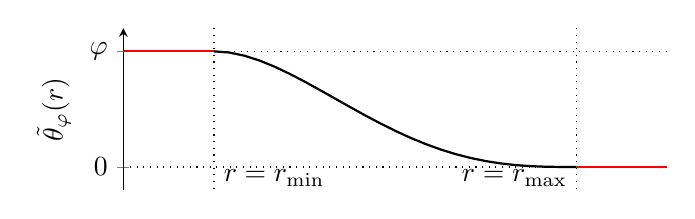
\begin{tikzpicture}
      \begin{axis}[
        ylabel={$\tilde{\theta}_\varphi(r)$},
        width=0.7\textwidth,
        height=0.3\textwidth,
        axis lines=left,
        hide x axis,
        ymin=-0.2, ymax=1.2,
        ytick={0,1},
        yticklabels={$0$,$\varphi$},
        ]
        \addplot[thick, red, domain=0:1] {1};
        \addplot[thick, red, domain=5:6] {0};
        \addplot[thick, domain=1:5] {(1-((x-1)/4))^3 * (3*(x-1)/4+1)};
        \draw[dotted] (axis cs:1,1.2) -- (axis cs:1,-0.2);
        \draw[dotted] (axis cs:5,1.2) -- (axis cs:5,-0.2);
        \draw[dotted] (axis cs:0,0) -- (axis cs:5,0);
        \draw[dotted] (axis cs:1,1) -- (axis cs:6,1);
        \node[anchor=south west] at (axis cs:1,-0.25) {$r=r_\text{min}$};
        \node[anchor=south east] at (axis cs:5,-0.25) {$r=r_\text{max}$};
      \end{axis}
    \end{tikzpicture}
  \end{center}
  \caption{$\tilde{\theta}_\varphi(r)$ as a function of $r$.}
  \label{fig:thetatilde}
\end{figure}

It is desirable that the entire airfoil is contained within the region $r <
r_\text{min}$, and that the boundary of the mesh is entirely inside the region
$r > r_\text{max}$. Given these restrictions, the mesh may otherwise be freely
chosen.

In the following we will denote by $\theta(r)$ a \emph{canonical} angle
function, satisfying
\[
  \theta(r) = \begin{cases}
    1, & r \le r_\text{min}, \\
    0, & r \ge r_\text{max}.
  \end{cases}
\]
With this, we can write $\tilde{\theta}_\varphi(r) = \varphi \theta(r)$.
The mapping from reference coordinates to physical coordinates can then be
expressed as
\[
  \pi_{\varphi}^{-1} \hat{\bm r}
  = \bm R(\varphi \theta(r)) \; \hat{\bm r},
\]
where $\hat{\bm r} = \left( \hat{x}, \hat{y} \right)$,
$r = \| \hat{\bm r} \| = \sqrt{\hat{x}^2 + \hat{y}^2}$
and $\bm R$ is the rotation matrix,
\[
  \bm R(a) = \begin{pmatrix} \cos a & - \sin a \\ \sin a & \cos a \end{pmatrix}.
\]

The Jacobian $\bm J = \bm J(\pi_{\varphi}^{-1})$ can be expressed,
using $a = \varphi \theta(r)$ as shorthand, as
\begin{align}
  \nonumber
  \bm J &= \bm R(a) + \bm R'(a) \hat{\bm r} \nabla a^\intercal
  = \bm R(a) \left( \bm I + \bm P \hat{\bm r} \nabla a^\intercal \right) \\
  &= \bm R(a) \left(
    \bm I + \frac{\varphi \theta'}{r} \bm P \hat{\bm r} \hat{\bm r}^\intercal
  \right)
  = \bm R(a) \left( \bm I + \varphi \bm P \bm Q \right)
\end{align}
where $\bm R'(a) = \partial \bm R(a) / \partial a$ and
where the two utility matrices $\bm P$ and $\bm Q$ are defined as
\begin{equation}
  \bm P = \bm R(\nicefrac{\pi}{2}), \qquad
  \bm Q = \frac{\theta'}{r} \hat{\bm r} \hat{\bm r}^\intercal,
\end{equation}
noting the useful property that $\bm R \bm P = \bm R'$.

The determinant of $\bm R$ is $1$ and the determinant of $\bm J$ follows
from the matrix determinant lemma (as a one-rank update to an invertible
matrix),
\[
  \det \bm J = 1 + \frac{\varphi\theta'}{r} \hat{\bm r}^\intercal \bm P \hat{\bm r} = 1,
\]
since the last term may be recognized as the inner product between two
orthogonal vectors.

The inverse of $\bm J$ follows from the Sherman-Morrison theorem,
\[
  \bm J^{-1} = \left( \bm I - \varphi \bm P \bm Q \right)
  \bm R(a)^\intercal.
\]

It can then be seen that the problem of finding affine representations of
$\bm J$ and $\bm J^{-1}$ reduces to the affine representation of $\bm R$.
We therefore proceed as follows.
\[
  \bm R(a)
  = \begin{pmatrix} \cos a & -\sin a \\ \sin a & \cos a \end{pmatrix}
  = \sum_{i=0}^\infty \left( \frac{(-1)^i a^{2i}}{(2i)!} \bm I
    + \frac{(-1)^i a^{2i+1}}{(2i+1)!} \bm P \right).
\]
Noting that, since $\bm P^0 = \bm I$, $\bm P^1 = \bm P$, $\bm P^2 = -\bm I$,
$\bm P^3 = -\bm P$ etc., we obtain
\[
  (-1)^i \bm I = \bm P^{2i}, \qquad (-1)^i \bm P = \bm P^{2i+1},
\]
so the series expansion can be more succinctly written as
\begin{equation}
  \label{eqn:rotsum}
  \bm R(a) = \sum_{i=0}^\infty \frac{a^i}{i!} \bm P^i
  = \sum_{i=0}^\infty \varphi^i \underbrace{\frac{\theta^i}{i!}\bm P^i}_{\bm R_i}
  = \sum_{i=0}^\infty \varphi^i \bm R_i.
\end{equation}

To investigate the effect of the Piola transformation, we consider the affine
representations \eqref{eqn:split-1}--\eqref{eqn:split-3} for two different
methods. First, a conventional method using the pullback $\pi_{\bm \mu}^*$ to
map between function spaces, and second a divergence-conforming method based on
the Piola mapping \eqref{eqn:piola}.

In doing so we will truncate the series for $\bm R(a)$ to a number of terms that
can achieve the desired precision. It is important to note that the system
\eqref{eqn:piolablock} only obtains its desired form for high accuracy
approximations, and that if the affine representation form for
$b(\cdot,\cdot,\bm \mu)$ is not exact, the matrix $\bm B_{vp}$ from
\eqref{eqn:block} will correspondingly not be exactly zero, and the solution of
\eqref{eqn:blocksolve-1}--\eqref{eqn:blocksolve-2} will not agree with the
solution of \eqref{eqn:block}.

The error made by truncating \eqref{eqn:rotsum} to $n$ terms is approximately
$\varphi_\text{max}^n / n!$. For a maximal angle of attack of
$\SI{35}{\degree}$ for example, we can expect about $10$ digits of accuracy
with $n=10$ terms.

In the following, only the parameter $\varphi$ is treated, as $u_\infty$ is
comparatively trivial.

\subsection{Non-Piola formulation}

For the laplacian form $d$ we get
\begin{align}
  d(
    \pi_{\varphi}^* \hat{\bm u},
    \pi_{\varphi}^* \hat{\bm w};
    \varphi
  )
  &= \nu \int_{\hat{\Omega}} (\bm J^{-\intercal} \nabla) \hat{\bm u} : (\bm J^{-\intercal} \nabla) \hat{\bm w}
  = \nu \int_{\hat{\Omega}} \nabla \hat{\bm u} : (\bm J^{-1} \bm J^{-\intercal} \nabla) \hat{\bm w},
\end{align}
and we find for the matrix $\bm J^{-1} \bm J^{-\intercal}$ that
\begin{align}
  \nonumber
  \bm J^{-1} \bm J^{-\intercal}
  &= (\bm I - \varphi \bm P \bm Q) \bm R^\intercal
    \bm R (\bm I + \varphi \bm Q \bm P) \\
  \nonumber
  &= \bm I + \varphi \underbrace{(\bm Q \bm P - \bm P \bm Q)}_{\bm D_1}
    - \varphi^2 \underbrace{\bm P \bm Q^2 \bm P}_{\bm D_2} \\
  &= \bm I + \varphi \bm D_1 - \varphi^2 \bm D_2.
\end{align}
Giving a three-term affine representation of $d$ as
\begin{equation}
  d(
    \pi_{\varphi}^* \hat{\bm u},
    \pi_{\varphi}^* \hat{\bm w};
    \varphi
  ) =
  \nu \int_{\hat{\Omega}} \nabla \hat{\bm u} : \nabla \hat{\bm w}
  + \nu \varphi \int_{\hat{\Omega}}
  \nabla \hat{\bm u} : (\bm D_1 \nabla) \hat{\bm w}
  - \nu \varphi^2 \int_{\hat{\Omega}}
  \nabla \hat{\bm u} : (\bm D_2 \nabla) \hat{\bm w}.
\end{equation}

For the divergence form $b$ we have
\begin{equation}
  b(
    \pi_{\varphi}^* \hat{p},
    \pi_{\varphi}^* \hat{\bm w};
    \varphi
  ) =
  \int_{\hat{\Omega}} \hat{p} (\bm J^{-\intercal} \nabla) \cdot \hat{\bm w}
  = \int_{\hat{\Omega}} \hat{p} \bm J^{-\intercal} : \nabla \hat{\bm w},
\end{equation}
meaning we need a series representation of $\bm J^{-\intercal}$:
\begin{align}
  \nonumber
  \bm J^{-\intercal}
  &= \bm R(a) (\bm I - \varphi \bm Q^\intercal \bm P^\intercal)
  = \bm R(a) (\bm I + \varphi \bm Q \bm P)
  = \sum_{i=0}^\infty
    \varphi^i \bm R_i
    (\bm I + \varphi \bm Q \bm P) \\
  &= \sum_{i=0}^\infty
    \varphi^i \bm R_i
    + \varphi^{i+1} \bm R_i \bm Q \bm P
  = \sum_{i=0}^\infty
    \varphi^i \underbrace{\left(
    \bm R_i + \bm R_{i-1} \bm Q \bm P
    \right)}_{\bm B^{(-)}_i}
  = \sum_{i=0}^\infty \varphi^i \bm B^{(-)}_i,
\end{align}
with the understanding that $\bm R_{-1} = 0$. This gives an affine
representation of $b$ in $2n$ terms, where $n$ is a suitable number of terms for
a truncated Taylor series for $\sin$ or $\cos$, given the range of $\varphi$
under consideration.
\begin{equation}
  b(
    \pi_{\varphi}^* \hat{p},
    \pi_{\varphi}^* \hat{\bm w};
    \varphi
  ) \approx \sum_{i=0}^{2n} \varphi^i
  \int_{\hat{\Omega}} \hat{p} \bm B^{(-)}_i : \nabla \hat{\bm w}
\end{equation}

The same expansion will work with the convective term $c$, viz.
\begin{equation}
  c(
    \pi_{\varphi}^* \hat{\bm u},
    \pi_{\varphi}^* \hat{\bm v},
    \pi_{\varphi}^* \hat{\bm w};
    \varphi
  )
  = \int_{\hat{\Omega}} (\hat{\bm u} \cdot \bm J^{-\intercal}\nabla) \hat{\bm v} \cdot \hat{\bm w}
  \approx \sum_{i=0}^{2n} \varphi^i \int_{\hat{\Omega}}
    (\hat{\bm u} \cdot \bm B^{(-)}_i \nabla) \hat{\bm v} \cdot \hat{\bm w}.
\end{equation}

\subsection{Piola formulation}

This proceeds as for the non-Piola case, except every vector field is
pre-multiplied with the Jacobian (recall, the determinant is $1$, which
simplifies \eqref{eqn:piola} somewhat). For this, we need an affine
representation of $\bm J$. It looks deceptively like that of $\bm
J^{-\intercal}$.
\begin{align}
  \nonumber
  \bm J
  &= \bm R(a) (\bm I + \varphi \bm P \bm Q)
  = \sum_{i=0}^\infty \varphi^i \bm R_i (\bm I + \varphi \bm P \bm Q)
  = \sum_{i=0}^\infty \varphi^i \bm R_i + \varphi^{i+1} \bm P \bm Q \\
  &= \sum_{i=0}^\infty
    \varphi^i \underbrace{\left(
    \bm R_i + \bm R_{i-1} \bm P \bm Q
    \right)}_{\bm B^{(+)}_i} = \sum_{i=0}^\infty \varphi^i \bm B^{(+)}_i.
\end{align}
For the form $b$ we then get
\begin{align}
  \nonumber
  b(
    \pi_{\varphi}^* \hat{p},
    \pi_{\varphi}^* \hat{\bm w};
    \varphi
  ) &= \int_{\hat{\Omega}} \hat{p} \bm J^{-\intercal} : \nabla (\bm J \hat{\bm w})
    \approx \int_{\hat{\Omega}} \hat{p}
      \left( \sum_{i=0}^{2n} \varphi^i \bm B^{(-)}_i \right) : \nabla
      \left( \sum_{j=0}^{2n} \varphi^j \bm B^{(+)}_j \hat{\bm w} \right) \\
    &= \sum_{i,j=0}^{2n} \varphi^{i+j}
      \int_{\hat{\Omega}} \hat{p} \bm B^{(-)}_i :
      \nabla \left( \bm B^{(+)}_j \hat{\bm w} \right).
\end{align}
Given truncated expressions for $\bm J$ and $\bm J^{-\intercal}$ with $2n$
terms, this is an affine representation with $4n$ terms.

The form $c$ has similar complexity.
\begin{align}
  \nonumber
  c(
    \pi_{\varphi}^* \hat{\bm u},
    \pi_{\varphi}^* \hat{\bm v},
    \pi_{\varphi}^* \hat{\bm w};
    \varphi
  )
  &= \int_{\hat{\Omega}} (\bm J \hat{\bm u} \cdot \bm J^{-\intercal}\nabla)
    \bm J \hat{\bm v} \cdot \bm J \hat{\bm w}
  \approx \int_{\hat{\Omega}} (\hat{\bm u} \cdot \nabla)
      \left( \sum_{i=0}^{2n} \varphi^i \bm B^{(+)}_i \hat{\bm v} \right) \cdot
    \left( \sum_{i=0}^{2n} \varphi^j \bm B^{(+)}_j \hat{\bm w} \right) \\
  &= \sum_{i,j=0}^{2n} \varphi^{i+j}
    \int_{\hat{\Omega}} (\hat{\bm u} \cdot \nabla) \bm B^{(+)}_i \hat{\bm v} \cdot \bm B^{(+)}_j \hat{\bm w}.
\end{align}

And finally, $d$ can be represented as
\begin{align}
  \nonumber
  d(
    \pi_{\varphi}^* \hat{\bm u},
    \pi_{\varphi}^* \hat{\bm w};
    \varphi
  ) &= \int_{\hat{\Omega}}
      (\bm J^{-\intercal} \nabla) (\bm J \hat{\bm u}) :
      (\bm J^{-\intercal} \nabla) (\bm J \hat{\bm w})
    = \int_{\hat{\Omega}}
      \nabla (\bm J \hat{\bm u}) :
      (\bm J^{-1} \bm J^{-\intercal} \nabla) (\bm J \hat{\bm w}) \\
  \nonumber
    &\approx \int_{\hat{\Omega}}
      \nabla \left( \sum_{i=0}^{2n} \varphi^i \bm B^{(+)}_i \hat{\bm u} \right) :
      ((\bm I + \varphi \bm D_1 - \varphi^2 \bm D_2) \nabla)
      \left( \sum_{j=0}^{2n} \varphi^j \bm B^{(+)}_j \hat{\bm w} \right) \\
  \nonumber
    &= \sum_{i,j=0}^{2n} \varphi^{i+j} \int_{\hat{\Omega}}
      \nabla (\bm B^{(+)}_i \hat{\bm u}) : \nabla (\bm B^{(+)}_j \hat{\bm w}) \\
  \nonumber
    &+ \sum_{i,j=0}^{2n} \varphi^{i+j+1} \int_{\hat{\Omega}}
      \nabla (\bm B^{(+)}_i \hat{\bm u}) : (\bm D_1 \nabla) (\bm B^{(+)}_j \hat{\bm w}) \\
    &- \sum_{i,j=0}^{2n} \varphi^{i+j+2} \int_{\hat{\Omega}}
      \nabla (\bm B^{(+)}_i \hat{\bm u}) : (\bm D_2 \nabla) (\bm B^{(+)}_j \hat{\bm w}),
\end{align}
which is an affine representation with $4n+2$ terms.

\section{Results}
\label{sec:results}

For both methods, an ensemble of 225 solutions was generated at the
$15 \times 15$ Gauss points for the parameter set
\[
  \mathcal{P} = \left\{ (\varphi,u_\infty) \;|\;
    \varphi \in [-\SI{35}{\degree},\SI{35}{\degree}],
    u_\infty \in [1, 20]
  \right\}.
\]
The viscosity was set at $\nu = \nicefrac{1}{6}$. The airfoil was chosen as a
NACA0015 profile with a chord length of $1$, thus giving an approximate maximal
Reynold's number of $120$.

The reference domain $\hat{\Omega}$ was chosen as a cylinder of radius $10$,
centered at the center of the airfoil. The mesh had $80$ elements in
the angular direction and $30$ elements in the radial direction. Given
discretization nodes $\{c_i\}_{i=1}^{80}$ for the airfoil, and
uniformly spaced nodes $\{b_i\}_{i=1}^{80}$ for the surrounding
circle, the interior nodes of the mesh were chosen as
\begin{equation}
  \label{eq:meshgen}
  d_{ij} = \left( \frac{j}{30} \right)^3 b_i +
  \left( 1 - \left( \frac{j}{30} \right)^3 \right) c_i
\end{equation}
providing an algebraically graded mesh with finer resolution near the airfoil.

The boundary conditions were enforced strongly at the inflow boundary,
with no-slip conditions on the airfoil and a do-nothing zero Neumann
boundary condition on the outflow. The lift function was chosen as the
solution to the Stokes problem with $\varphi=0$, which is solenoidal.

For parametrizing the geometry, the radius-dependent rotation angle function
$\theta$ was chosen as
\begin{align}
  \theta(r) = \begin{cases}
    1, & r < r_\text{min}, \\
    0, & r > r_\text{max}, \\
    (1-\overline{r})^3 (3\overline{r}+1), & \text{otherwise},
  \end{cases}
\end{align}
with
\[
  \overline{r} = \frac{(r - r_\text{min})}{(r_\text{max} - r_\text{min})},
  \qquad r_\text{min} = 1, \qquad r_\text{max} = 10,
\]
see Figures~\ref{fig:thetatilde} and \ref{fig:domain}.

\begin{figure}
  \begin{center}
    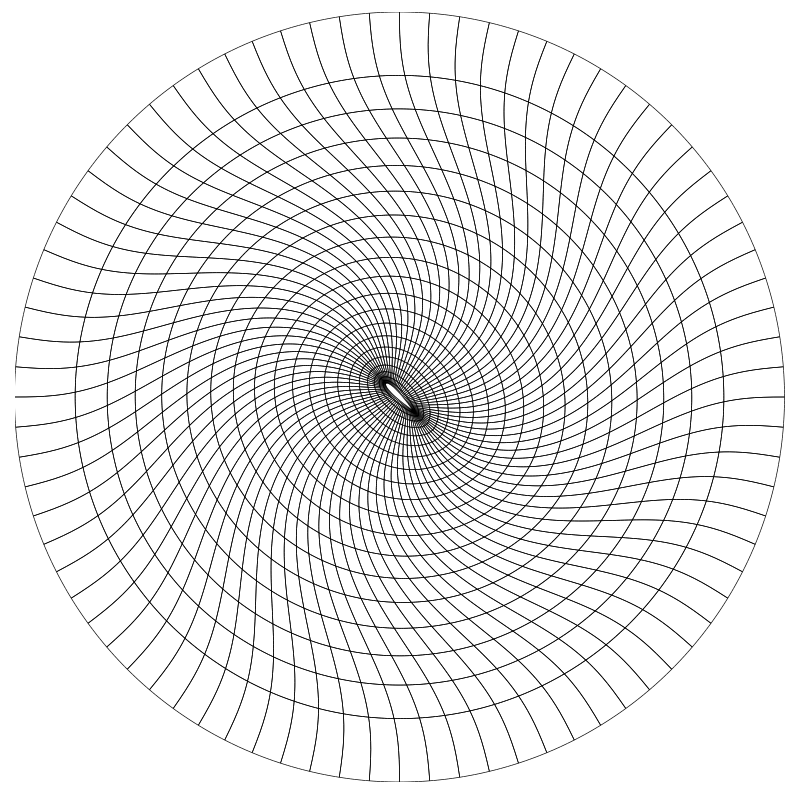
\includegraphics[width=0.5\textwidth]{figs/domain}
  \end{center}
  \caption{Sample domain with $\varphi = -\nicefrac{\pi}{4}$.}
  \label{fig:domain}
\end{figure}

For the regular high-fidelity mododel, we chose a Lagrangian quadratic basis for
velocity, and Lagrangian linear basis for the pressure. This fulfils the
Taylor-Hood property, leading to a stable method.

For the conforming high-fidelity model, we chose a quadratic B-spline basis for
the pressure, and a mixed cubic and quadratic B-spline basis for the velocity,
giving a fully divergence-conforming method for the reference geometry at
$\varphi=0$. Note that by design, the divergence-conforming method will retain
this property for other angles.

For solving the nonlinear equation we used Newton iteration, stopping when the
velocity update reached $10^{-10}$ or less, as measured in the $H^1$ seminorm.

The affine representations were derived from a truncated version of
\eqref{eqn:rotsum} with $n=12$ terms, sufficient to represent the rotation
matrix $\bm R(a)$ to $10$ digits accuracy within the range of angles considered.

Results have been generated for reduced models with $M=10,20,\ldots,50$ degrees
of freedom each in the three spaces (velocity, supremizers and pressure), as
well as the corresponding un-stabilized models (only velocity and pressure).
Additionally, for the conforming stabilized method, a distinction is made
between a naive solver and a block solver (see
\eqref{eqn:blocksolve-1}--\eqref{eqn:blocksolve-2}) where appropriate.

\subsection{Spectrum}

The decay rate of the eigenvalue spectrum of the solution ensembles indicate to
which degree one might expect a reduced basis to adequately capture the most
significant behavioral patterns of the model. As can be seen from
Figure~\ref{fig:spectra}, the decay is rapid for the first $20$ or so modes, and
then flattens out somewhat after that. (There is reason to believe that this
might be improved for different choices of $\theta$.) The spectra for the
supremizers closely mimic those of the pressure solutions, as should be
expected.

\begin{figure}
  \begin{tikzpicture}
    \begin{axis}[
      xlabel={$k$},
      ylabel={$\lambda_k$},
      ymode=log,
      xmin=0, xmax=225,
      width=0.9\textwidth,
      height=0.6\textwidth,
      grid=both,
      axis lines=left,
      legend style={
        at={(0.99, 0.98)},
        anchor=north east,
      },
      legend cell align=left,
      ]
      \addplot[red, thick]
      table[x index={0}, y index={1}]{data/airfoil-spectrum-no-piola.csv};
      \addplot[blue, thick]
      table[x index={0}, y index={2}]{data/airfoil-spectrum-no-piola.csv};
      \addplot[green, thick]
      table[x index={0}, y index={3}]{data/airfoil-spectrum-no-piola.csv};
      \addplot[red, thick, dashed]
      table[x index={0}, y index={1}]{data/airfoil-spectrum-piola.csv};
      \addplot[blue, thick, dashed]
      table[x index={0}, y index={2}]{data/airfoil-spectrum-piola.csv};
      \addplot[green, thick, dashed]
      table[x index={0}, y index={3}]{data/airfoil-spectrum-piola.csv};
      \legend{
        Regular ($v$),
        Regular ($p$),
        Regular (sup),
        Conforming ($v$),
        Conforming ($p$),
        Conforming (sup),
      }
    \end{axis}
  \end{tikzpicture}
  \caption{
    Ensemble spectra for 225 ensemble solutions for both methods, and all three
    spaces (velocity, pressure and supremizers).
  }
  \label{fig:spectra}
\end{figure}

\subsection{Basis functions}

The six dominant modes for for velocity, pressure and supremizers are shown. See
Figures~\ref{fig:modes-vel-noconf}--\ref{fig:modes-sup-noconf} for the regular
method and Figures~\ref{fig:modes-vel-conf}--\ref{fig:modes-sup-conf} for the
conforming method. As is common with reduced basis methods, we can see that the
first modes represent the most dominant flow patterns, and that it is left for
the higher order modes to represent finer details, in this case wake effects. It
is interesting that the first velocity modes of the two methods do not agree
(in fact, the second mode of the conforming method agrees with the first mode of
the regular method). The first two supremizer modes of the two methods also
appear to be ``switched''. As for the pressure modes, aside from sign flips,
they are in good agreement between the two methods, which is natural considering
that the function space mapping for the pressure is identical.

The divergences are shown in Figure~\ref{fig:divs}. Here, the \emph{mean} and
\emph{maximal} divergence of the ten first basis functions for each method
(measured in the $L^2$-norm) are shown for various angles of attack. It shows
that the divergences of the conforming basis functions are consistently zero to
$11$ or $12$ digits of accuracy (well within the $10$ digits chosen as a
baseline when choosing the number of terms $n$.) More importantly, it reveals
that the solenoidal property is consistently satisfied throughout the parameter
domain, with no significant variability.

\begin{figure}
  \begin{center}
    \adjustbox{trim={0.13\width} {0.12\height} {0.13\width} {0.12\height}, clip}{
      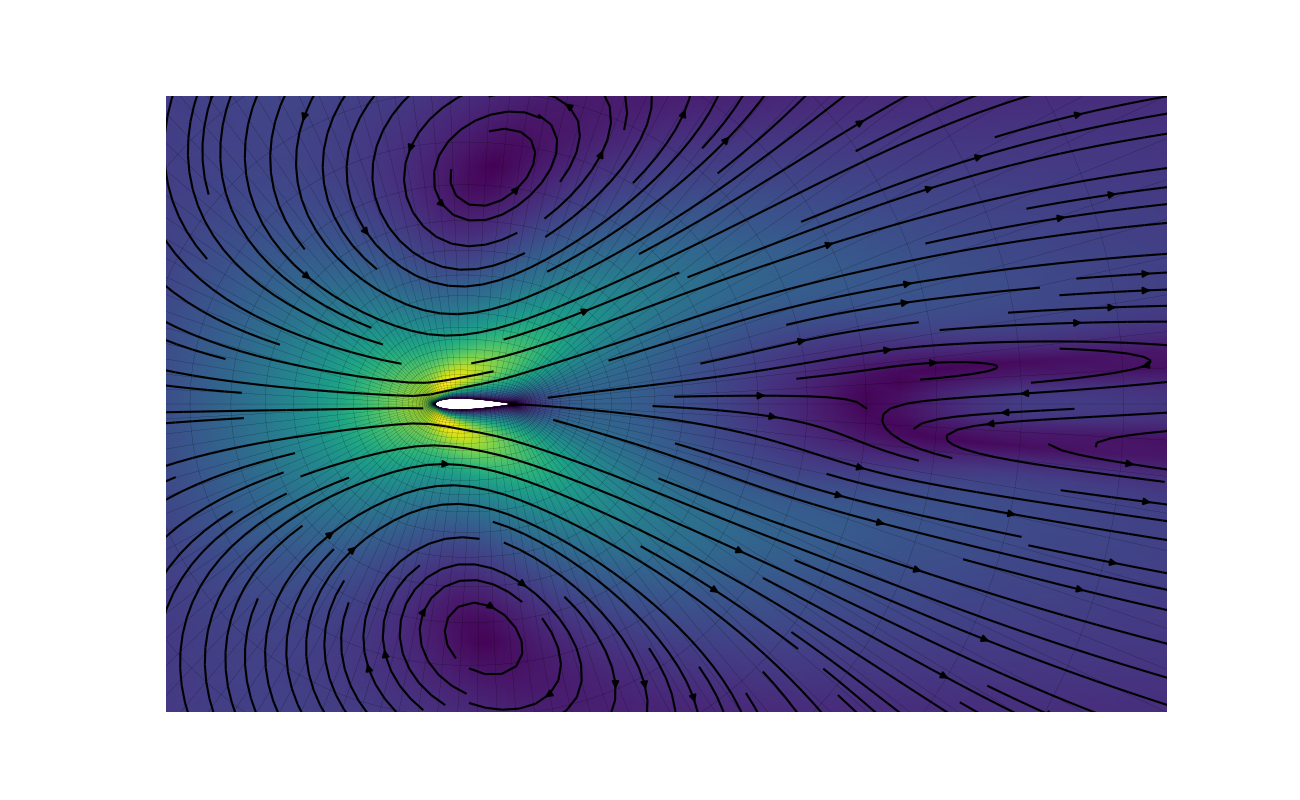
\includegraphics[width=0.4\textwidth]{figs/bfun-v-no-piola-v000}
    }
    \adjustbox{trim={0.13\width} {0.12\height} {0.13\width} {0.12\height}, clip}{
      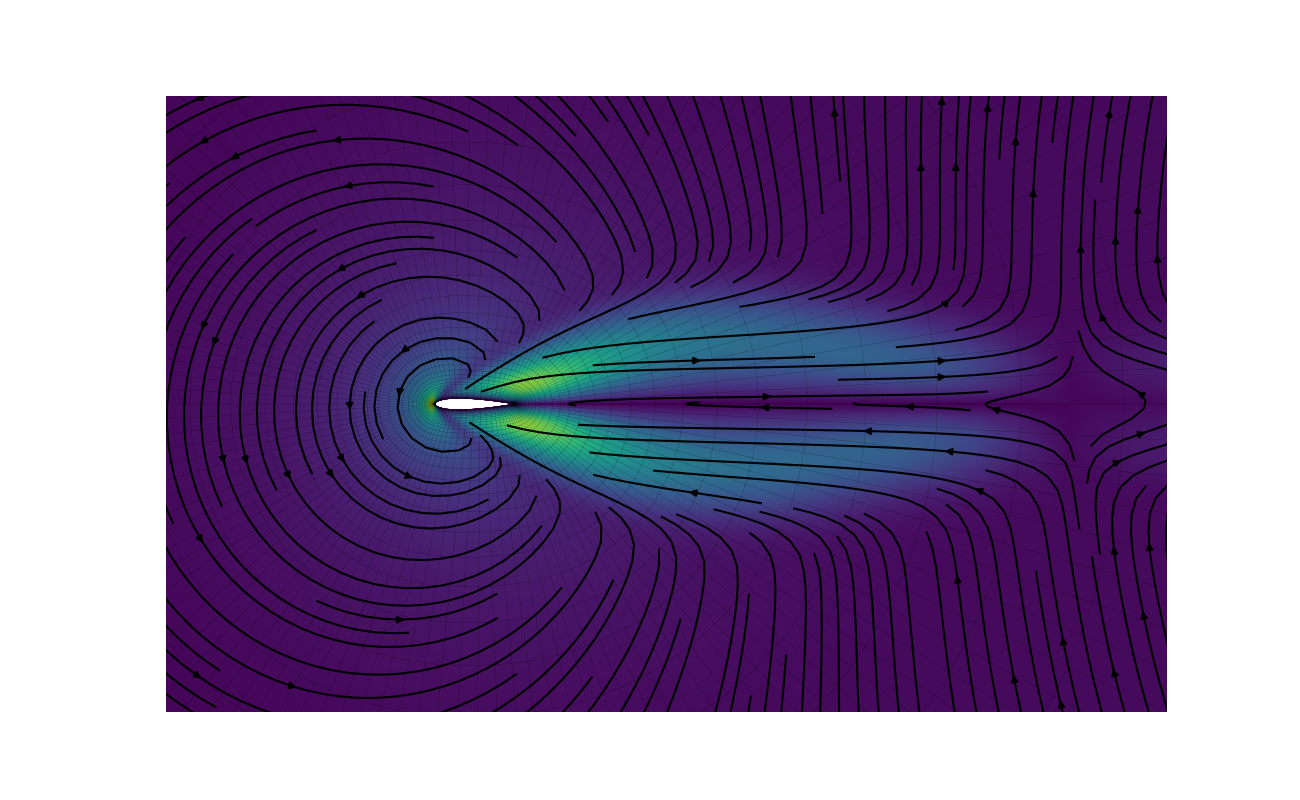
\includegraphics[width=0.4\textwidth]{figs/bfun-v-no-piola-v001}
    }
    \adjustbox{trim={0.13\width} {0.12\height} {0.13\width} {0.12\height}, clip}{
      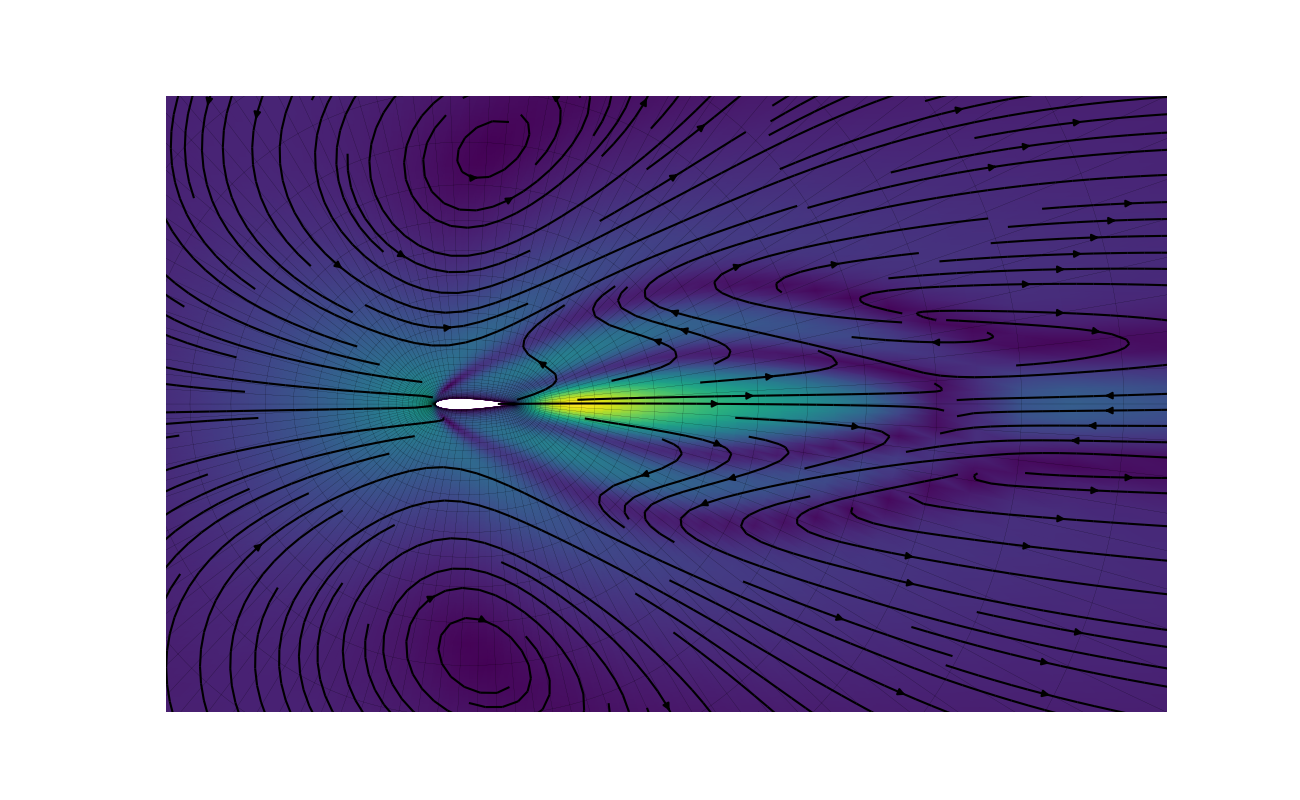
\includegraphics[width=0.4\textwidth]{figs/bfun-v-no-piola-v002}
    } \\
    \adjustbox{trim={0.13\width} {0.12\height} {0.13\width} {0.12\height}, clip}{
      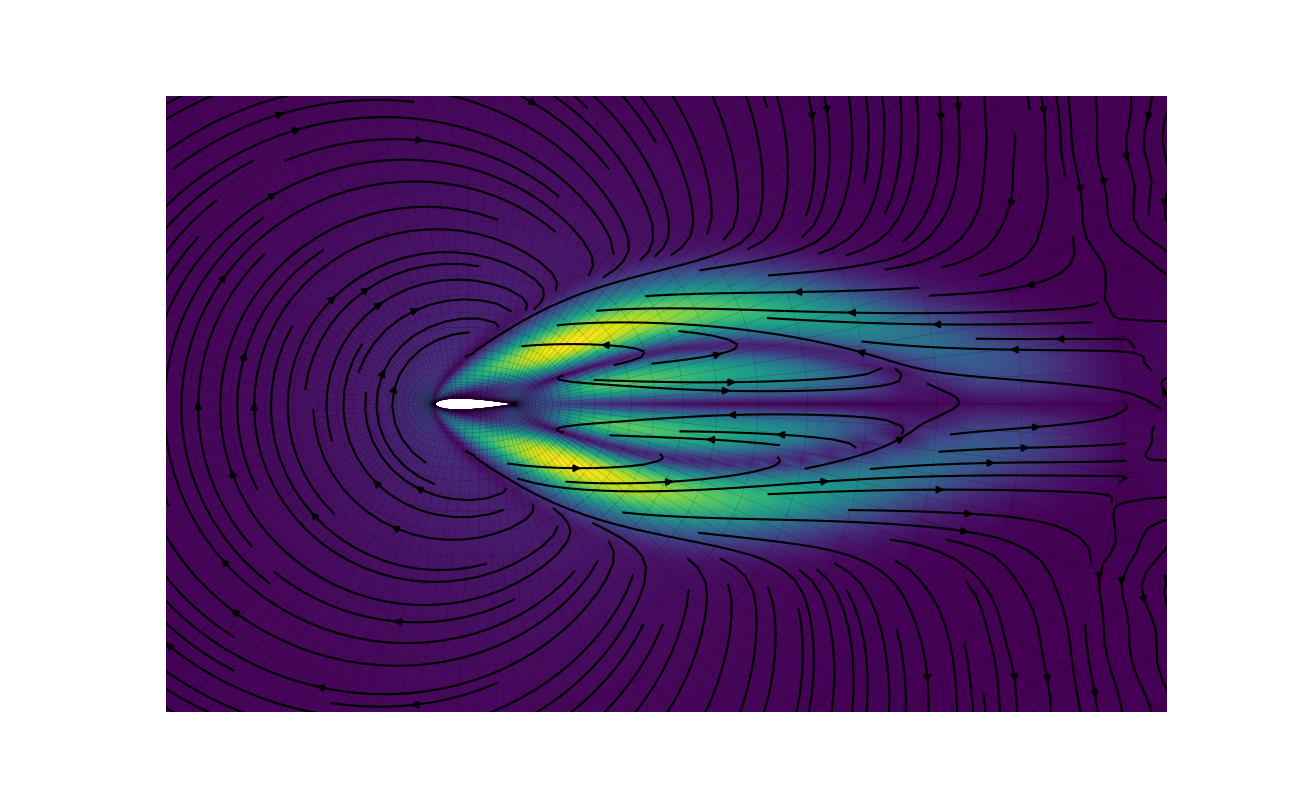
\includegraphics[width=0.4\textwidth]{figs/bfun-v-no-piola-v003}
    }
    \adjustbox{trim={0.13\width} {0.12\height} {0.13\width} {0.12\height}, clip}{
      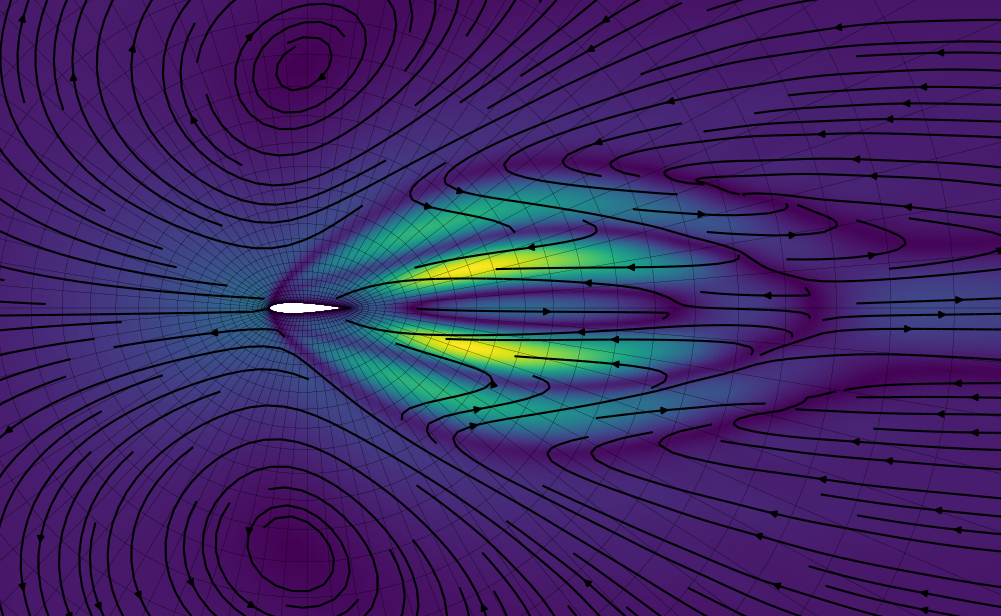
\includegraphics[width=0.4\textwidth]{figs/bfun-v-no-piola-v004}
    }
    \adjustbox{trim={0.13\width} {0.12\height} {0.13\width} {0.12\height}, clip}{
      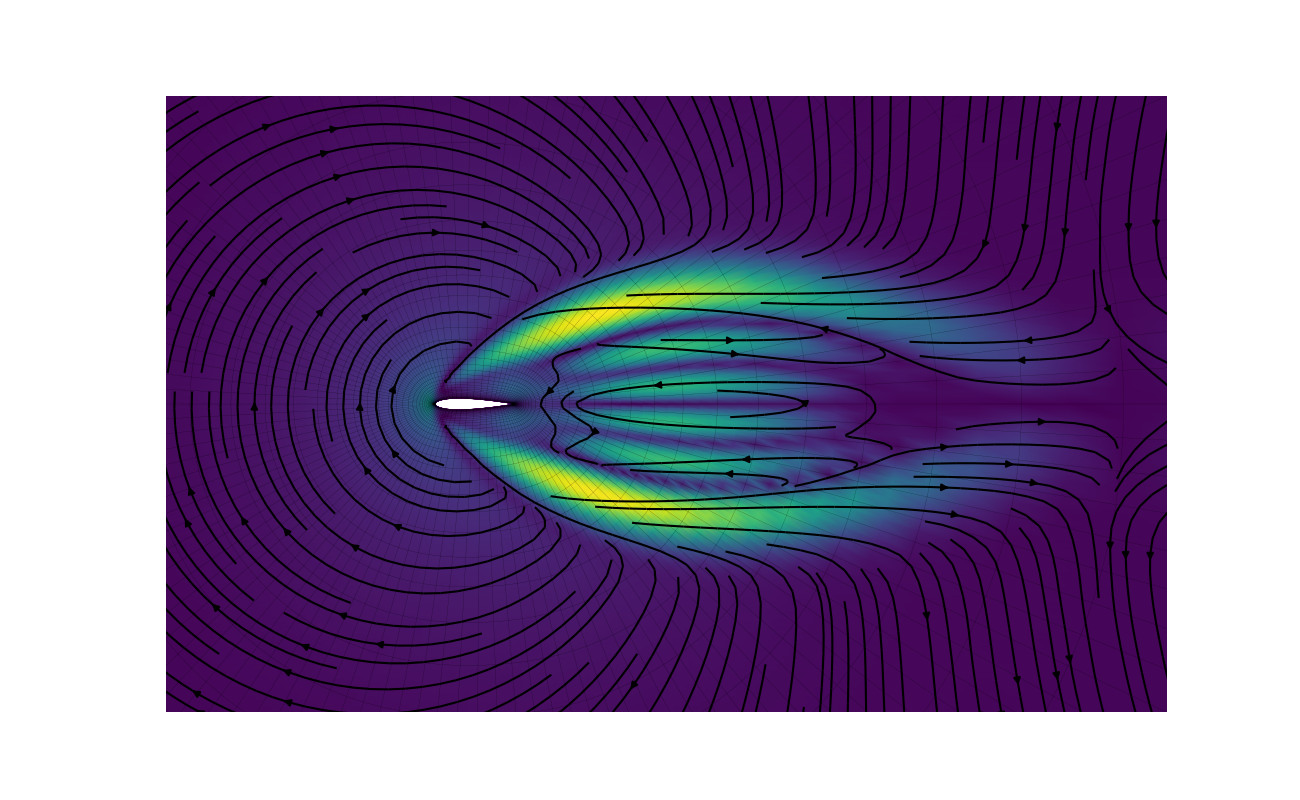
\includegraphics[width=0.4\textwidth]{figs/bfun-v-no-piola-v005}
    }
    \caption{First six velocity modes (regular method).}
    \label{fig:modes-vel-noconf}
  \end{center}
\end{figure}

\begin{figure}
  \begin{center}
    \adjustbox{trim={0.3\width} {0.3\height} {0.3\width} {0.3\height}, clip}{
      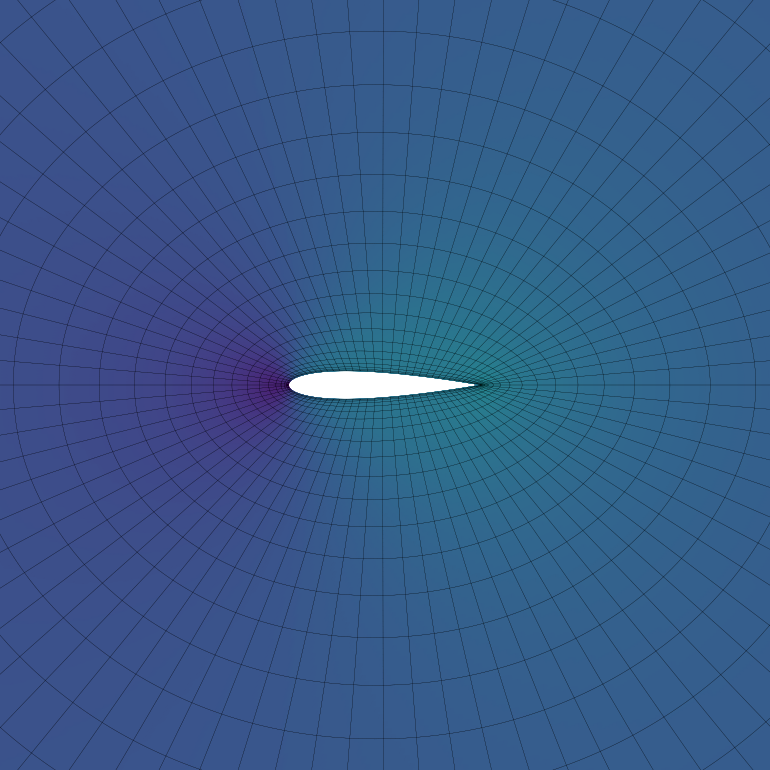
\includegraphics[width=0.4\textwidth]{figs/bfun-p-no-piola-p000}
    }
    \adjustbox{trim={0.3\width} {0.3\height} {0.3\width} {0.3\height}, clip}{
      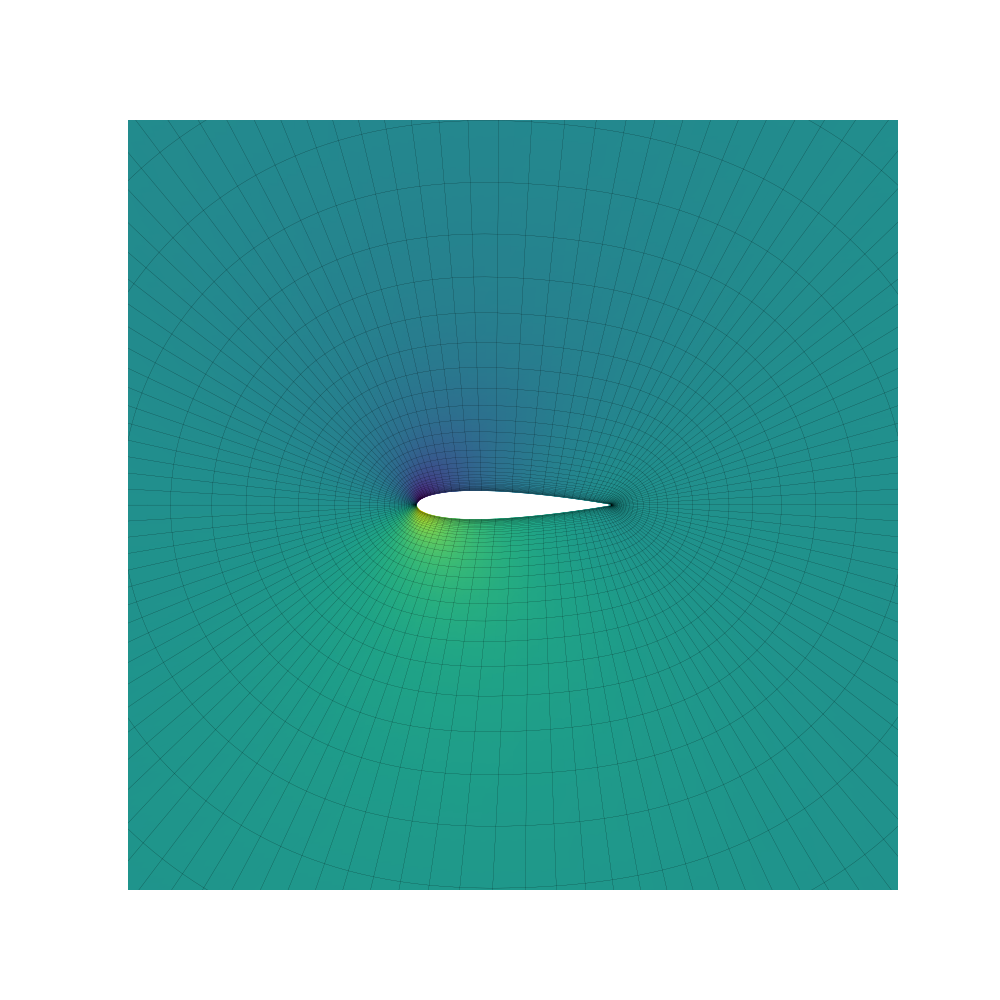
\includegraphics[width=0.4\textwidth]{figs/bfun-p-no-piola-p001}
    }
    \adjustbox{trim={0.3\width} {0.3\height} {0.3\width} {0.3\height}, clip}{
      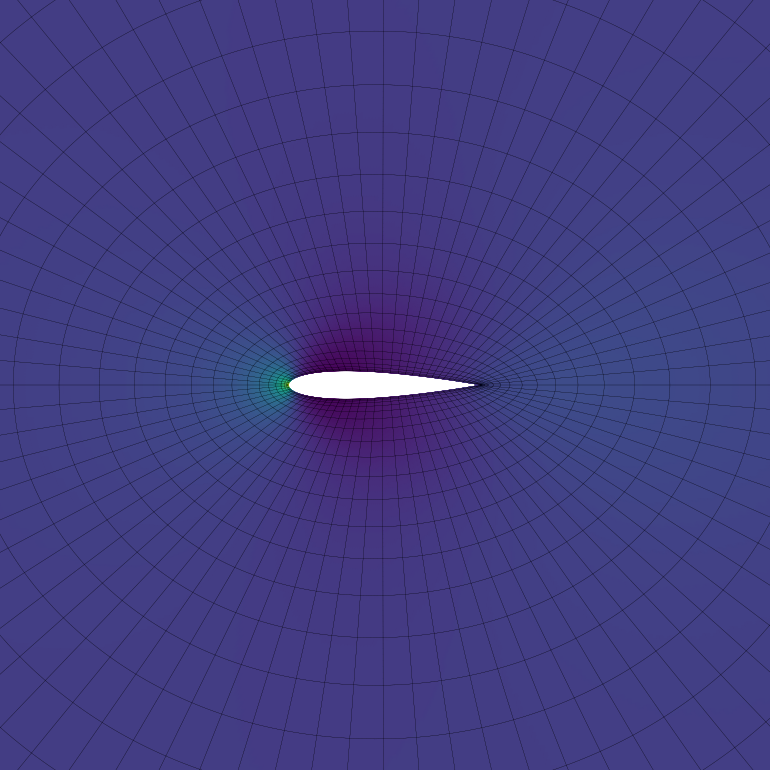
\includegraphics[width=0.4\textwidth]{figs/bfun-p-no-piola-p002}
    } \\
    \adjustbox{trim={0.3\width} {0.3\height} {0.3\width} {0.3\height}, clip}{
      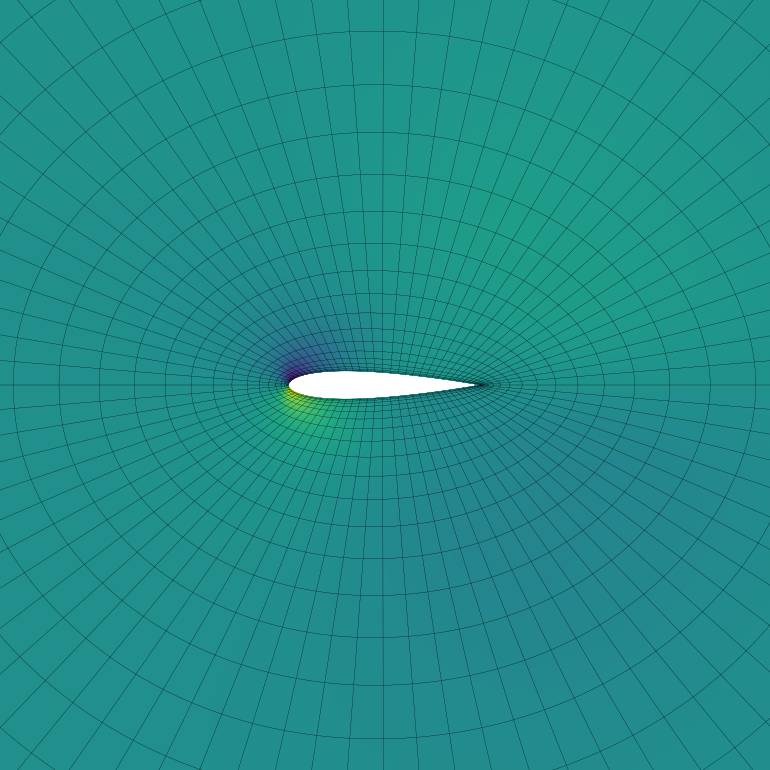
\includegraphics[width=0.4\textwidth]{figs/bfun-p-no-piola-p003}
    }
    \adjustbox{trim={0.3\width} {0.3\height} {0.3\width} {0.3\height}, clip}{
      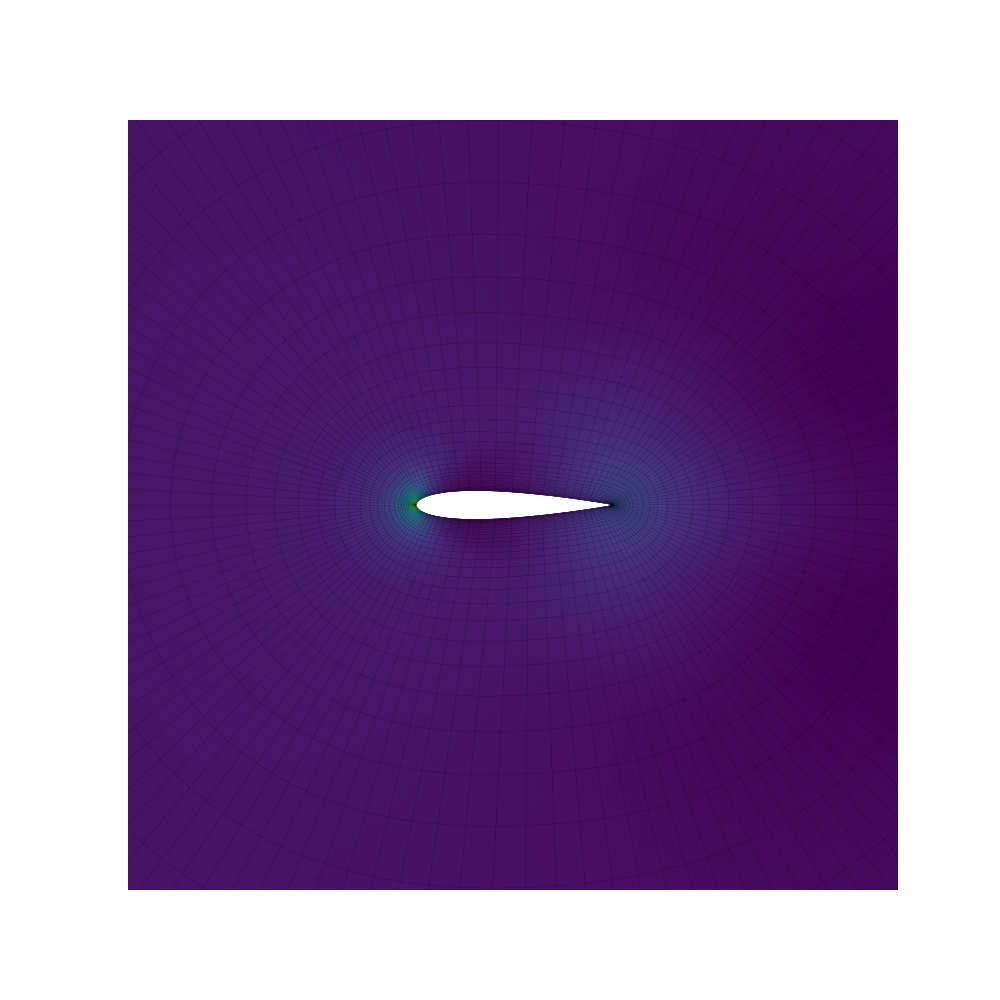
\includegraphics[width=0.4\textwidth]{figs/bfun-p-no-piola-p004}
    }
    \adjustbox{trim={0.3\width} {0.3\height} {0.3\width} {0.3\height}, clip}{
      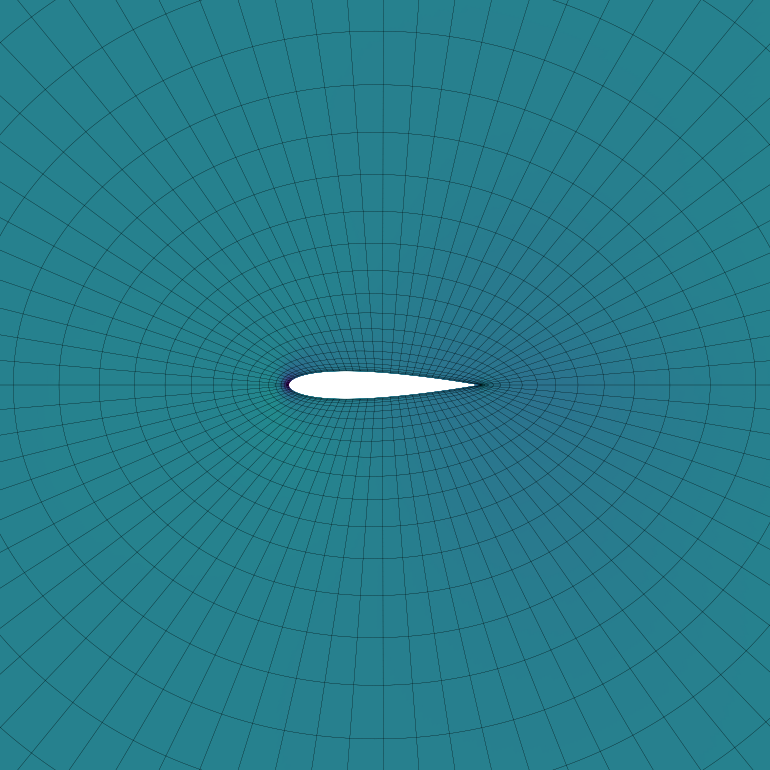
\includegraphics[width=0.4\textwidth]{figs/bfun-p-no-piola-p005}
    }
    \caption{First six pressure modes (regular method).}
    \label{fig:modes-press-noconf}
  \end{center}
\end{figure}

\begin{figure}
  \begin{center}
    \adjustbox{trim={0.2\width} {0.2\height} {0.2\width} {0.2\height}, clip}{
      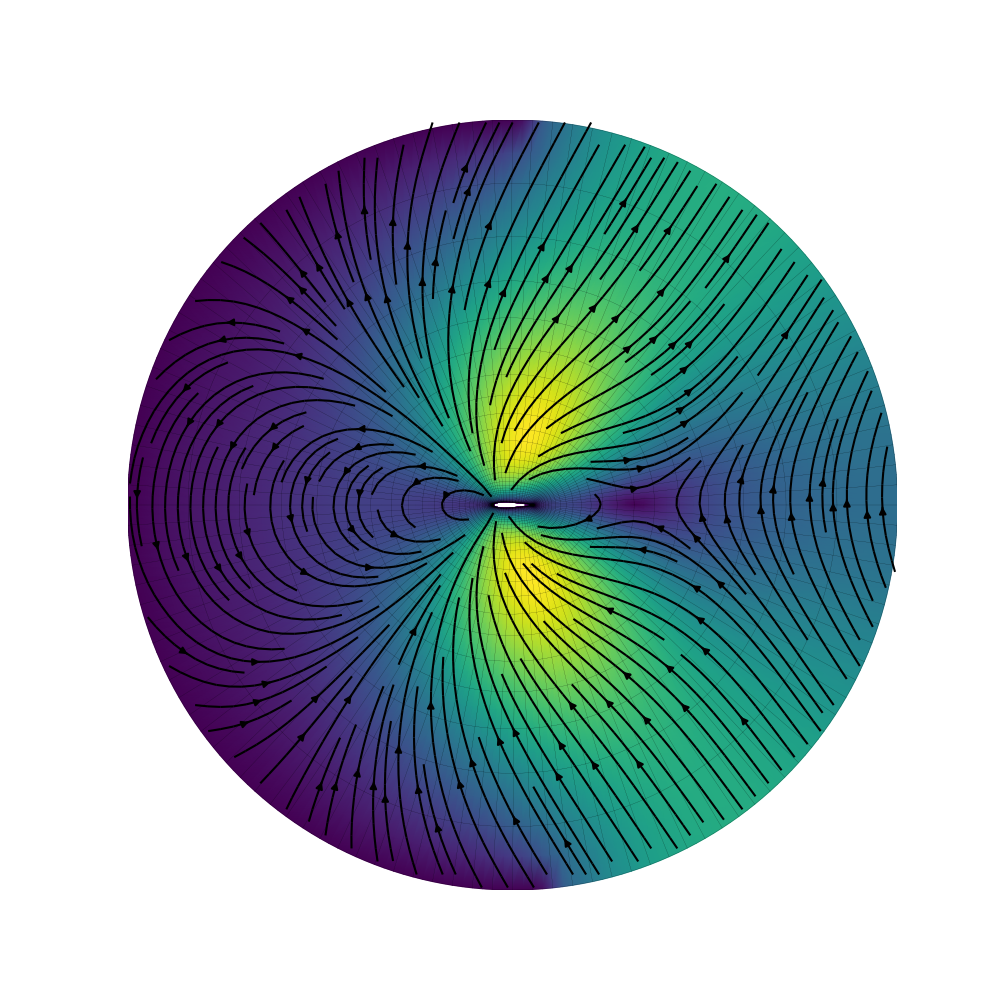
\includegraphics[width=0.4\textwidth]{figs/bfun-s-no-piola-v000}
    }
    \adjustbox{trim={0.2\width} {0.2\height} {0.2\width} {0.2\height}, clip}{
      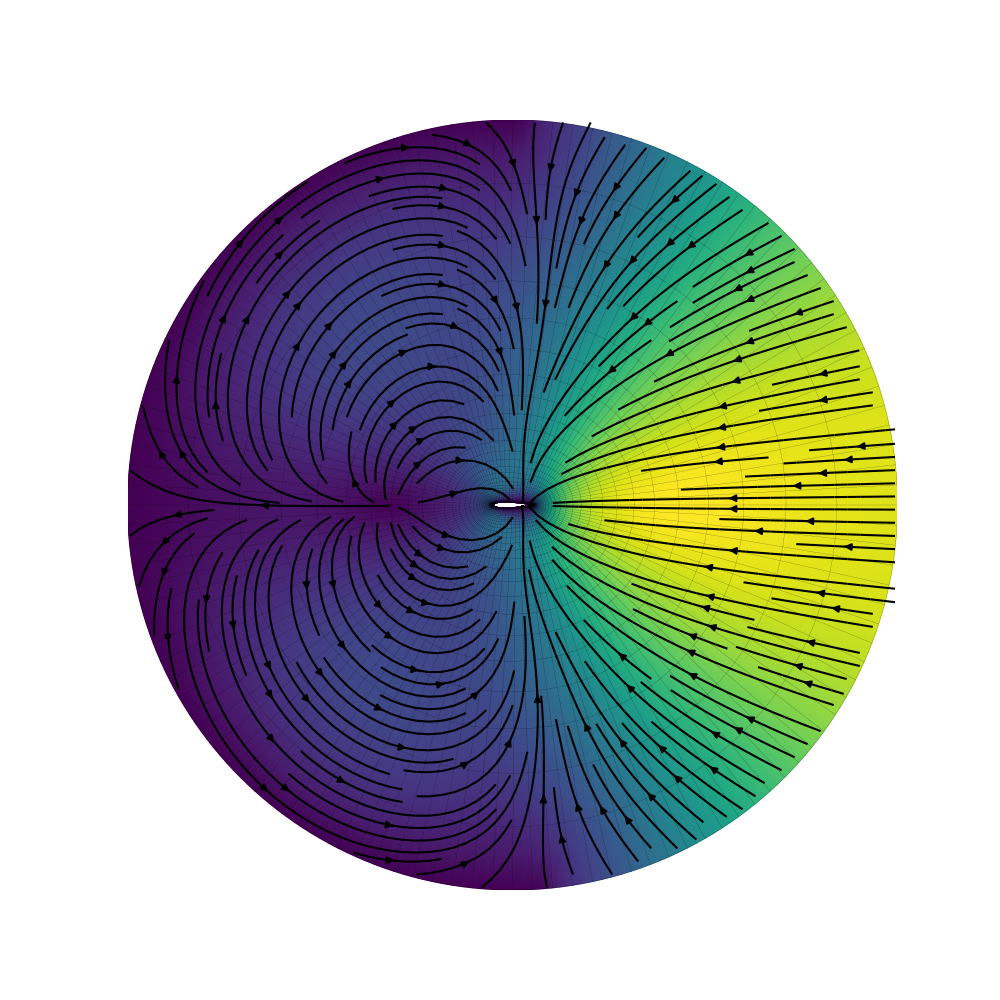
\includegraphics[width=0.4\textwidth]{figs/bfun-s-no-piola-v001}
    }
    \adjustbox{trim={0.2\width} {0.2\height} {0.2\width} {0.2\height}, clip}{
      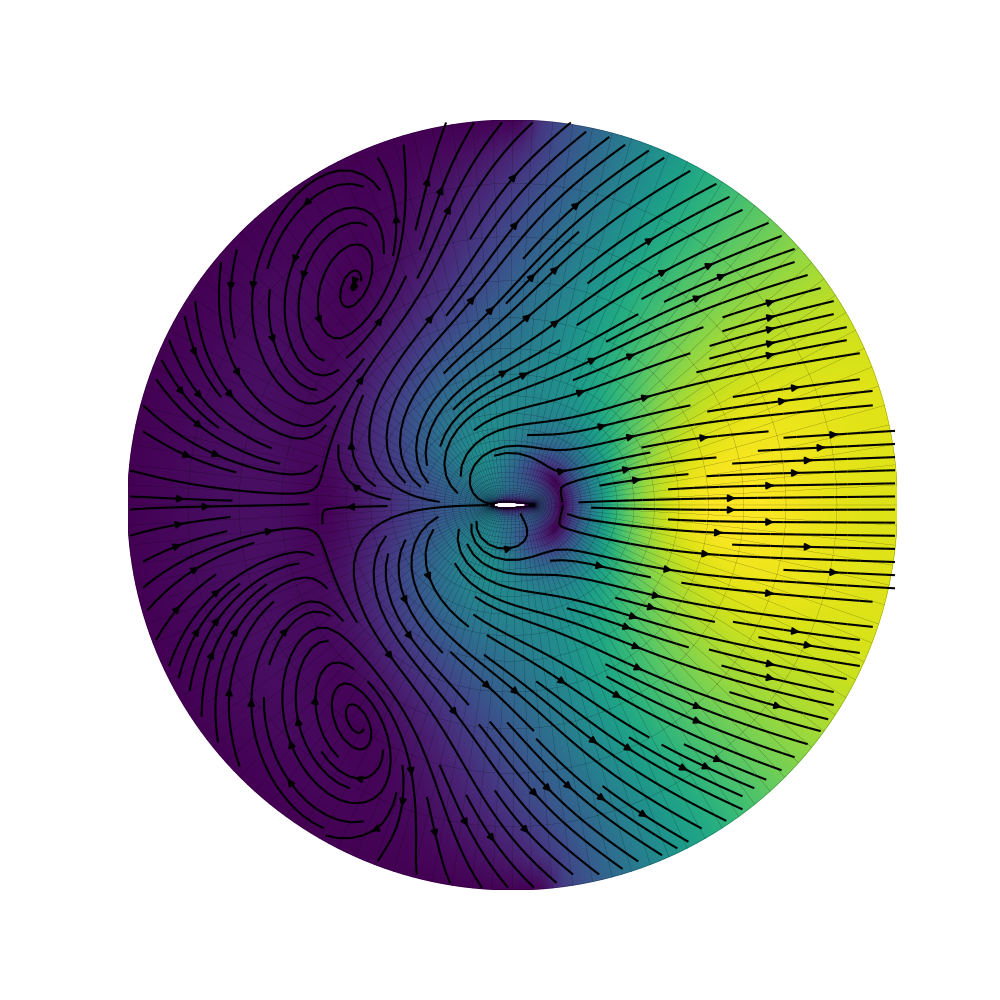
\includegraphics[width=0.4\textwidth]{figs/bfun-s-no-piola-v002}
    } \\
    \adjustbox{trim={0.2\width} {0.2\height} {0.2\width} {0.2\height}, clip}{
      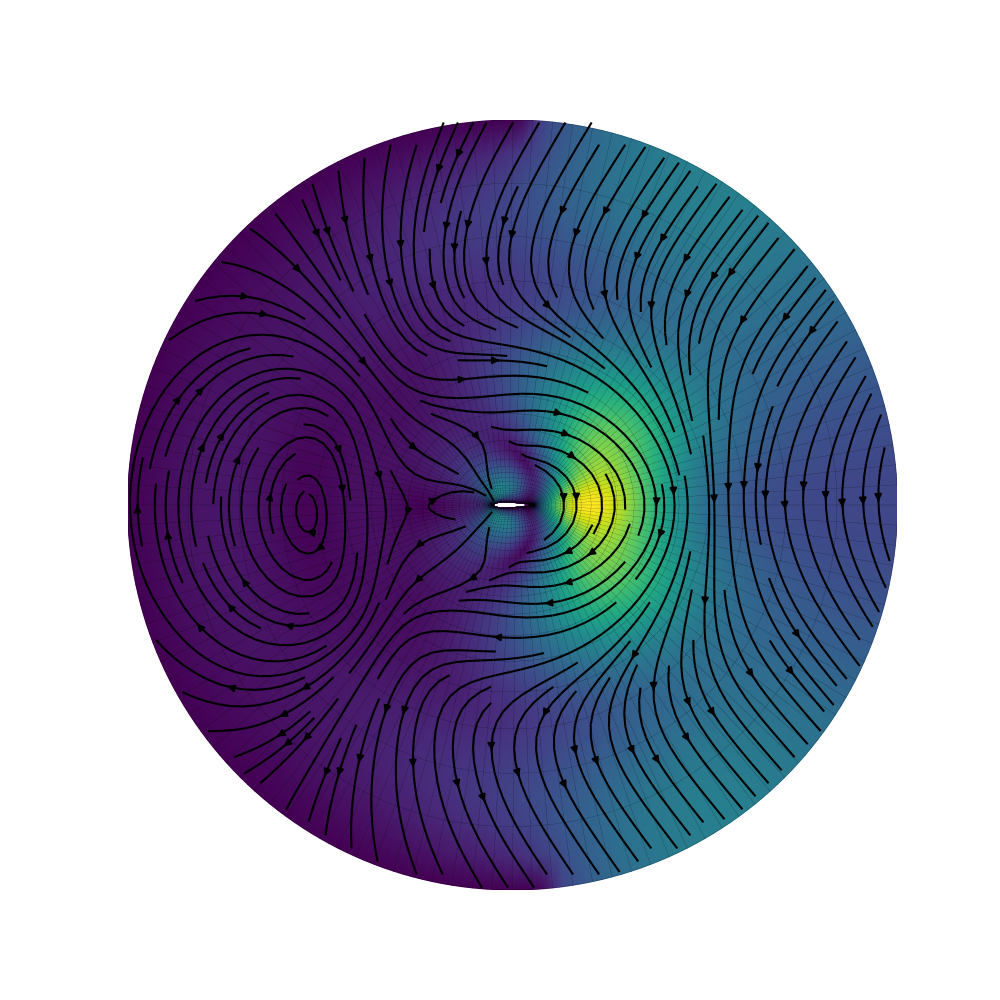
\includegraphics[width=0.4\textwidth]{figs/bfun-s-no-piola-v003}
    }
    \adjustbox{trim={0.2\width} {0.2\height} {0.2\width} {0.2\height}, clip}{
      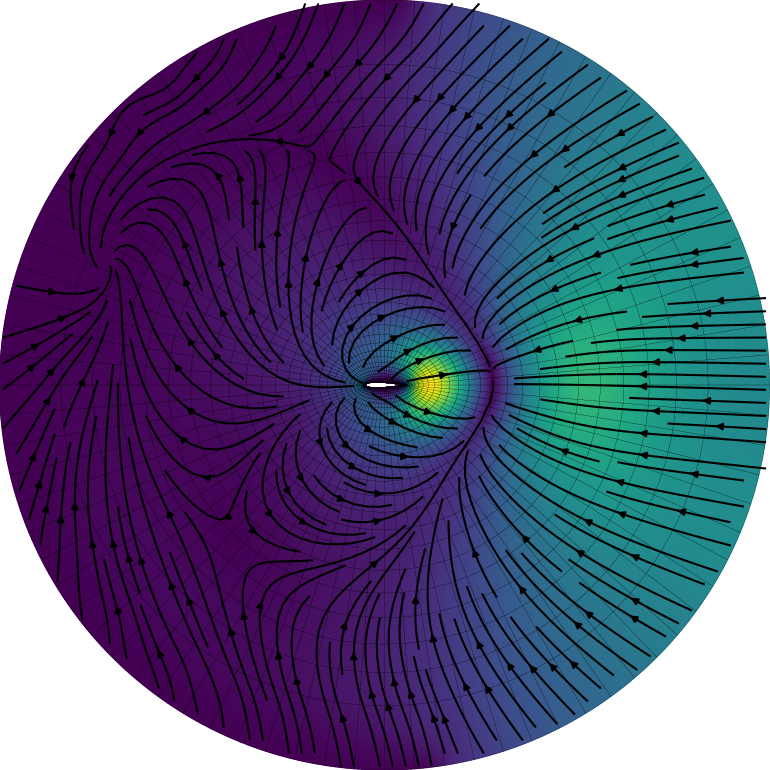
\includegraphics[width=0.4\textwidth]{figs/bfun-s-no-piola-v004}
    }
    \adjustbox{trim={0.2\width} {0.2\height} {0.2\width} {0.2\height}, clip}{
      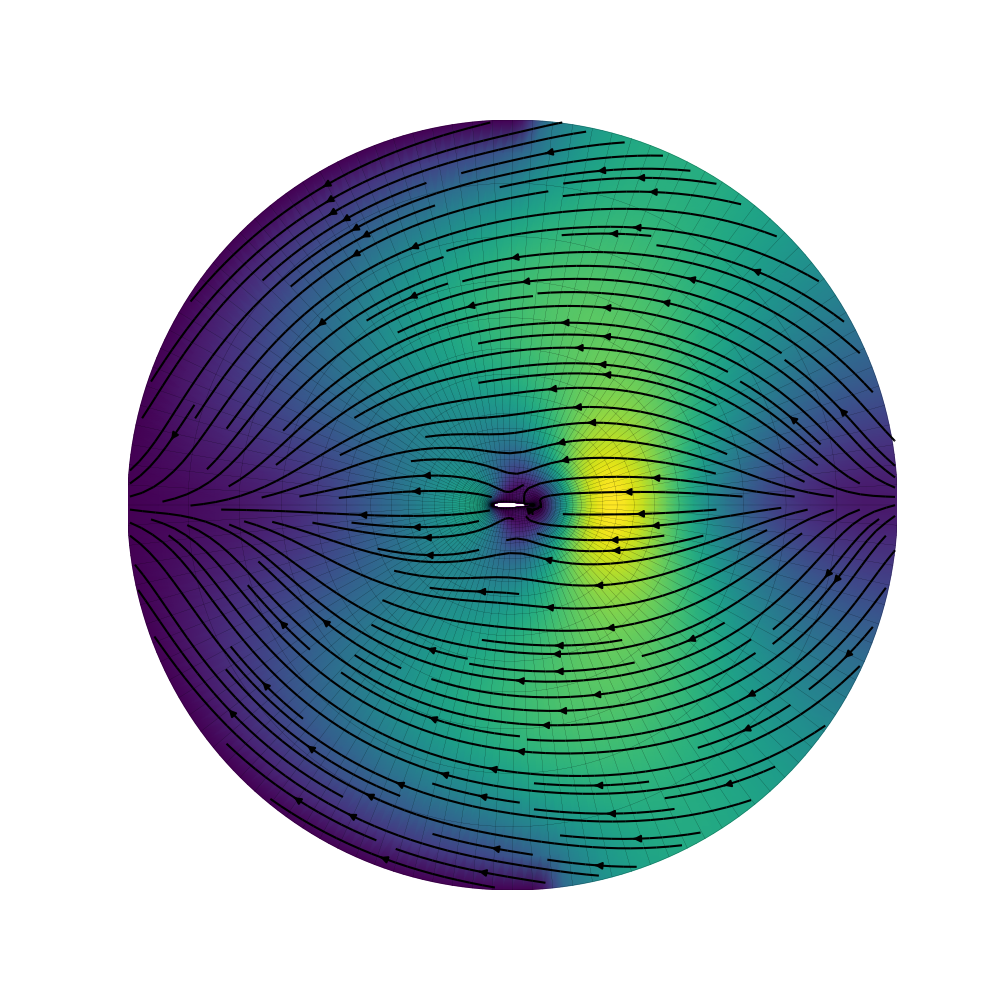
\includegraphics[width=0.4\textwidth]{figs/bfun-s-no-piola-v005}
    }
    \caption{First six supremizer modes (regular method).}
    \label{fig:modes-sup-noconf}
  \end{center}
\end{figure}

\begin{figure}
  \begin{center}
    \adjustbox{trim={0.13\width} {0.12\height} {0.13\width} {0.12\height}, clip}{
      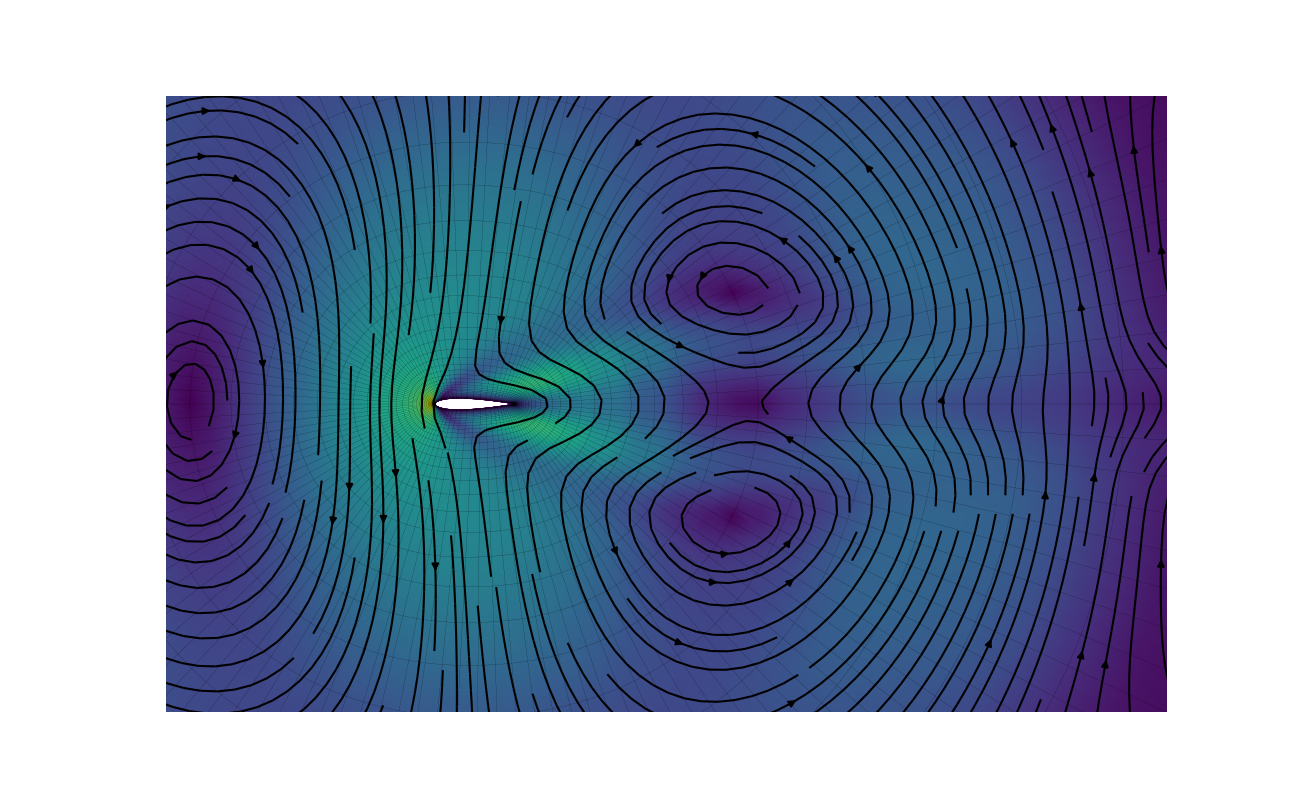
\includegraphics[width=0.4\textwidth]{figs/bfun-v-piola-v000}
    }
    \adjustbox{trim={0.13\width} {0.12\height} {0.13\width} {0.12\height}, clip}{
      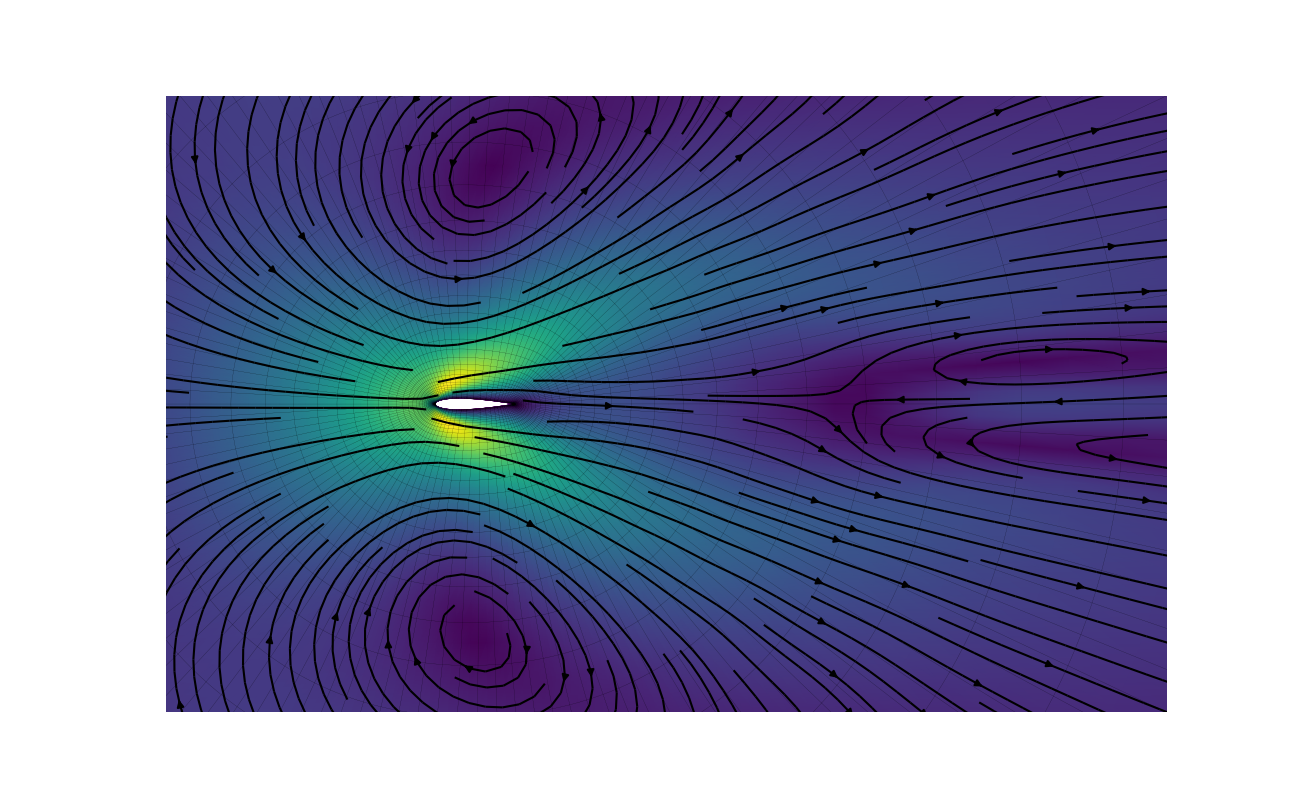
\includegraphics[width=0.4\textwidth]{figs/bfun-v-piola-v001}
    }
    \adjustbox{trim={0.13\width} {0.12\height} {0.13\width} {0.12\height}, clip}{
      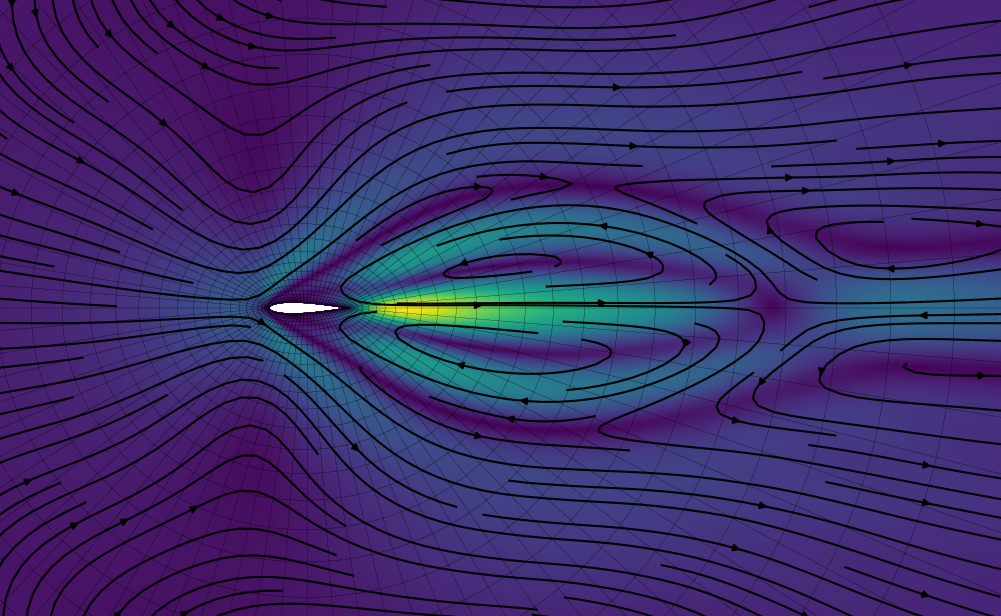
\includegraphics[width=0.4\textwidth]{figs/bfun-v-piola-v002}
    } \\
    \adjustbox{trim={0.13\width} {0.12\height} {0.13\width} {0.12\height}, clip}{
      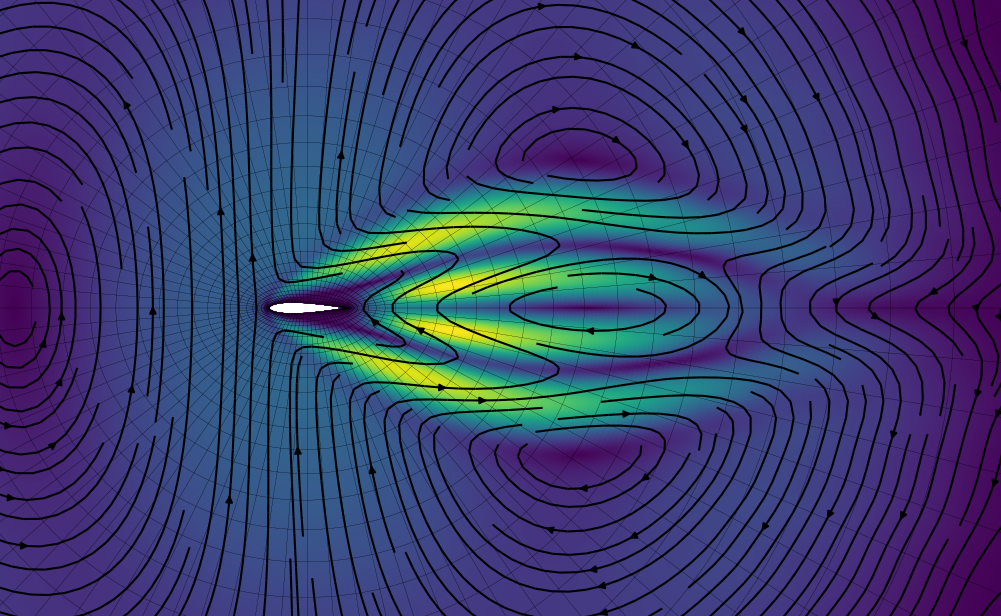
\includegraphics[width=0.4\textwidth]{figs/bfun-v-piola-v003}
    }
    \adjustbox{trim={0.13\width} {0.12\height} {0.13\width} {0.12\height}, clip}{
      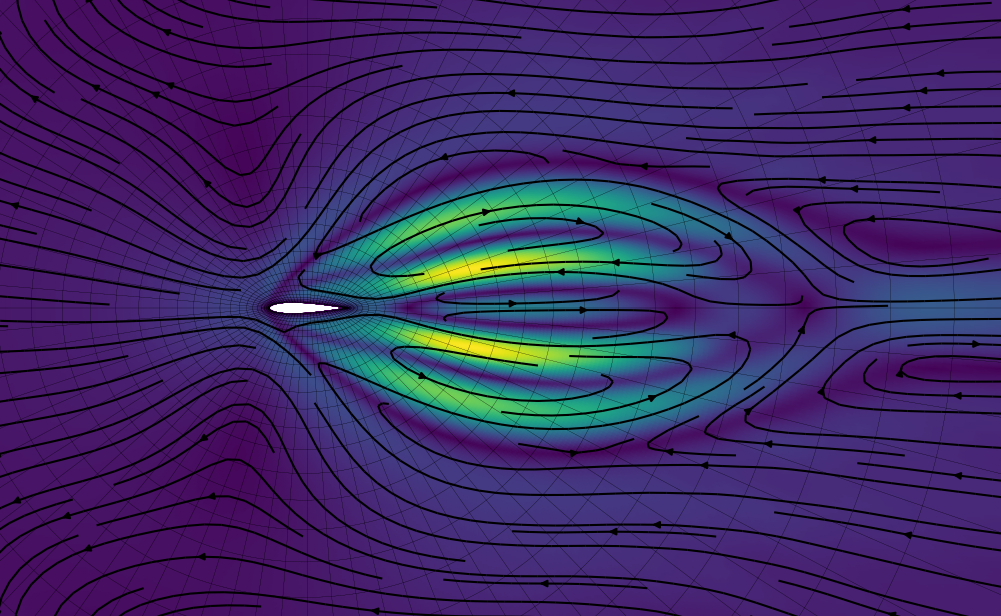
\includegraphics[width=0.4\textwidth]{figs/bfun-v-piola-v004}
    }
    \adjustbox{trim={0.13\width} {0.12\height} {0.13\width} {0.12\height}, clip}{
      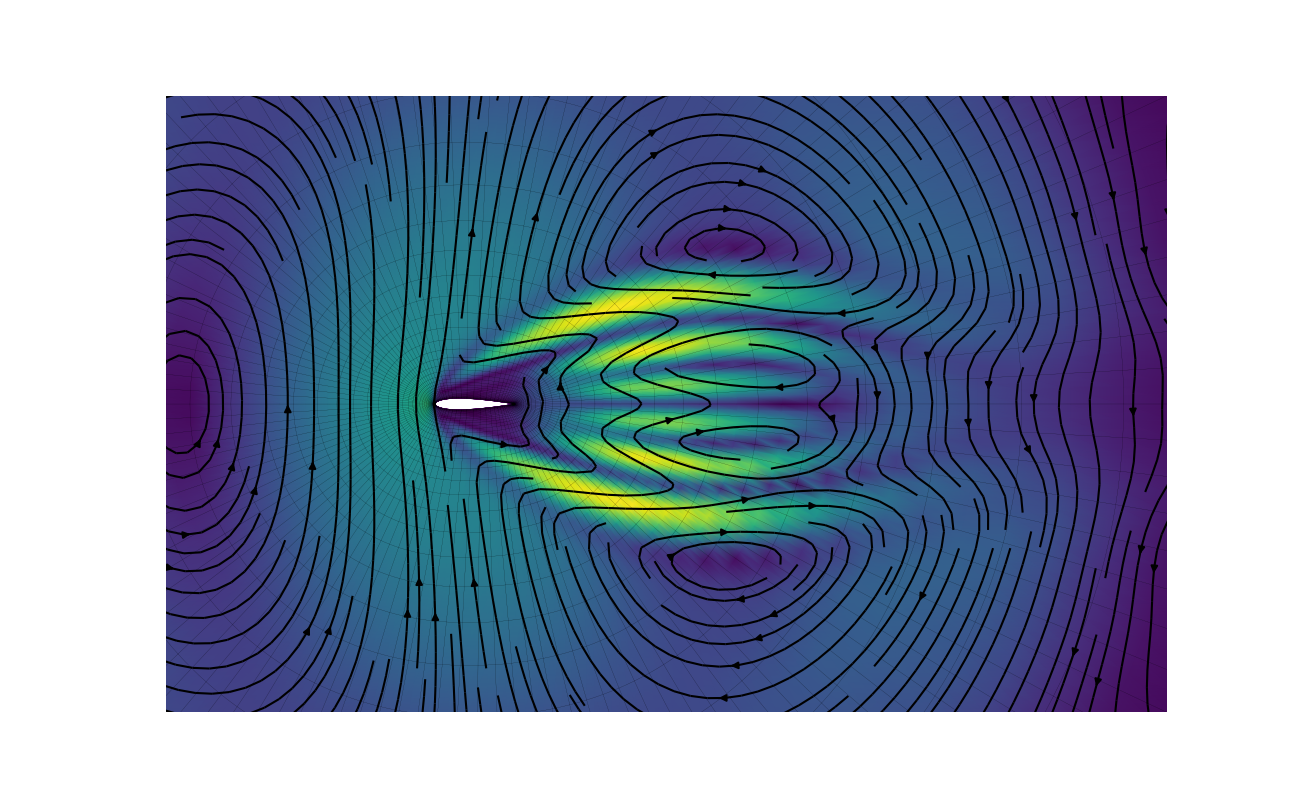
\includegraphics[width=0.4\textwidth]{figs/bfun-v-piola-v005}
    }
    \caption{First six velocity modes (conforming method).}
    \label{fig:modes-vel-conf}
  \end{center}
\end{figure}

\begin{figure}
  \begin{center}
    \adjustbox{trim={0.3\width} {0.3\height} {0.3\width} {0.3\height}, clip}{
      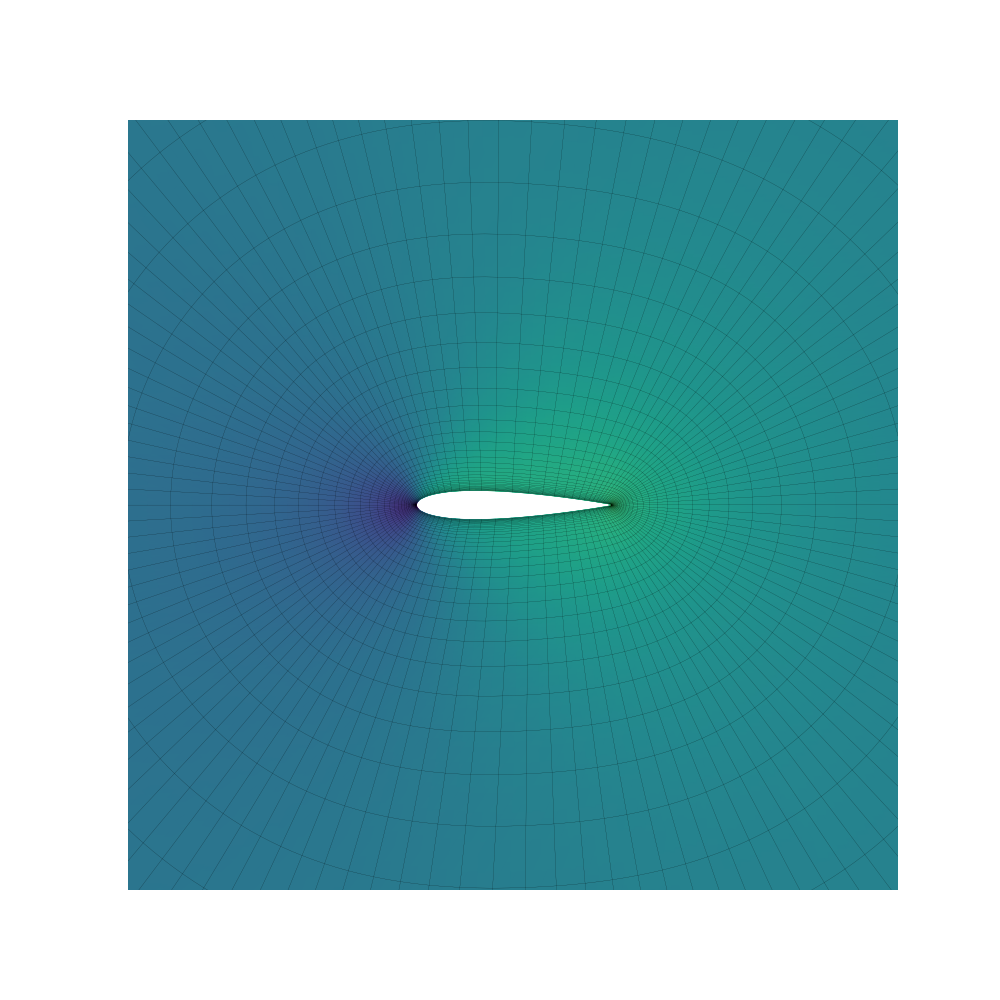
\includegraphics[width=0.4\textwidth]{figs/bfun-p-piola-p000}
    }
    \adjustbox{trim={0.3\width} {0.3\height} {0.3\width} {0.3\height}, clip}{
      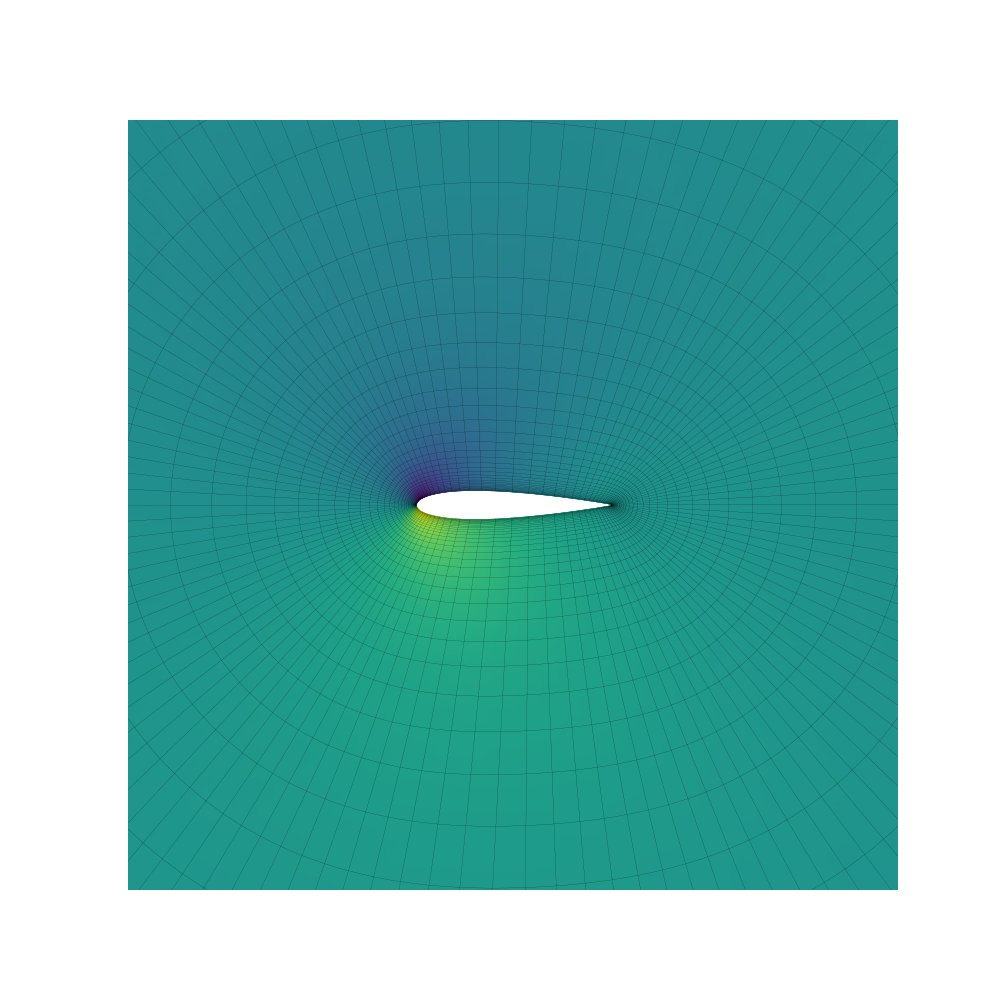
\includegraphics[width=0.4\textwidth]{figs/bfun-p-piola-p001}
    }
    \adjustbox{trim={0.3\width} {0.3\height} {0.3\width} {0.3\height}, clip}{
      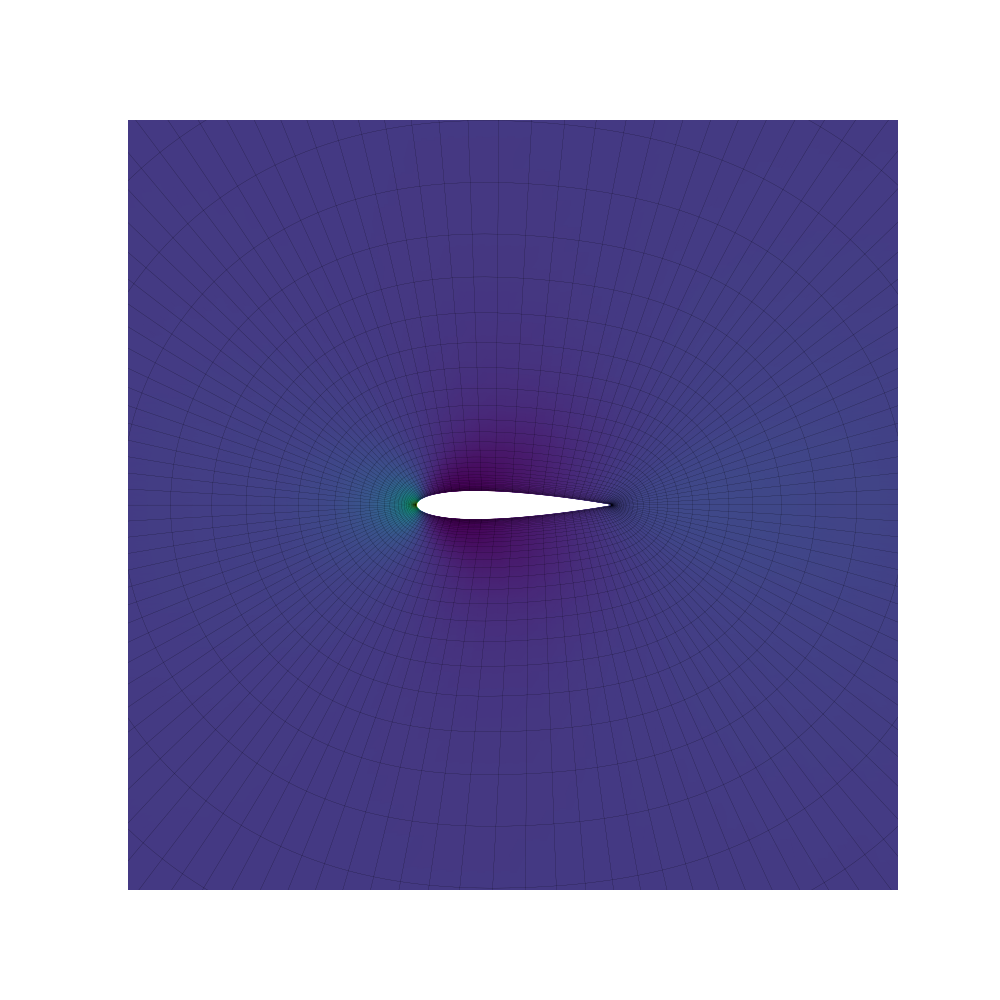
\includegraphics[width=0.4\textwidth]{figs/bfun-p-piola-p002}
    } \\
    \adjustbox{trim={0.3\width} {0.3\height} {0.3\width} {0.3\height}, clip}{
      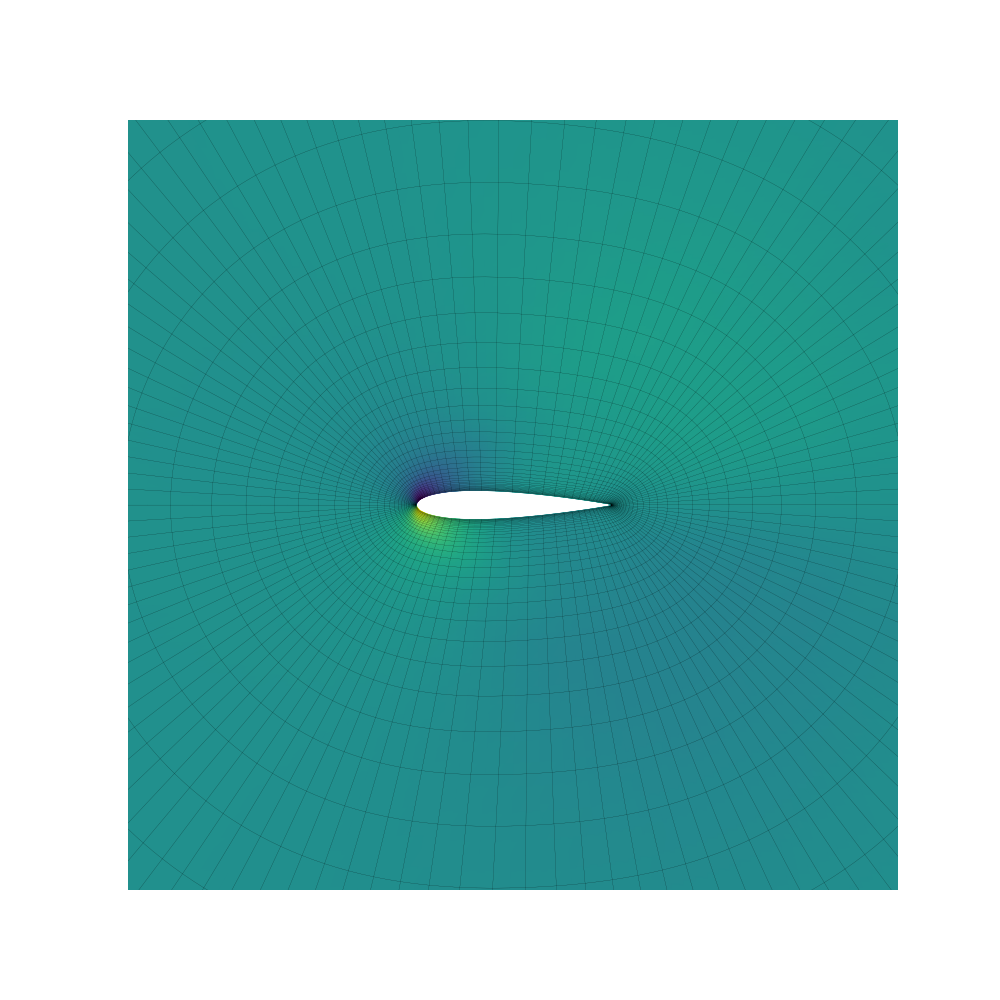
\includegraphics[width=0.4\textwidth]{figs/bfun-p-piola-p003}
    }
    \adjustbox{trim={0.3\width} {0.3\height} {0.3\width} {0.3\height}, clip}{
      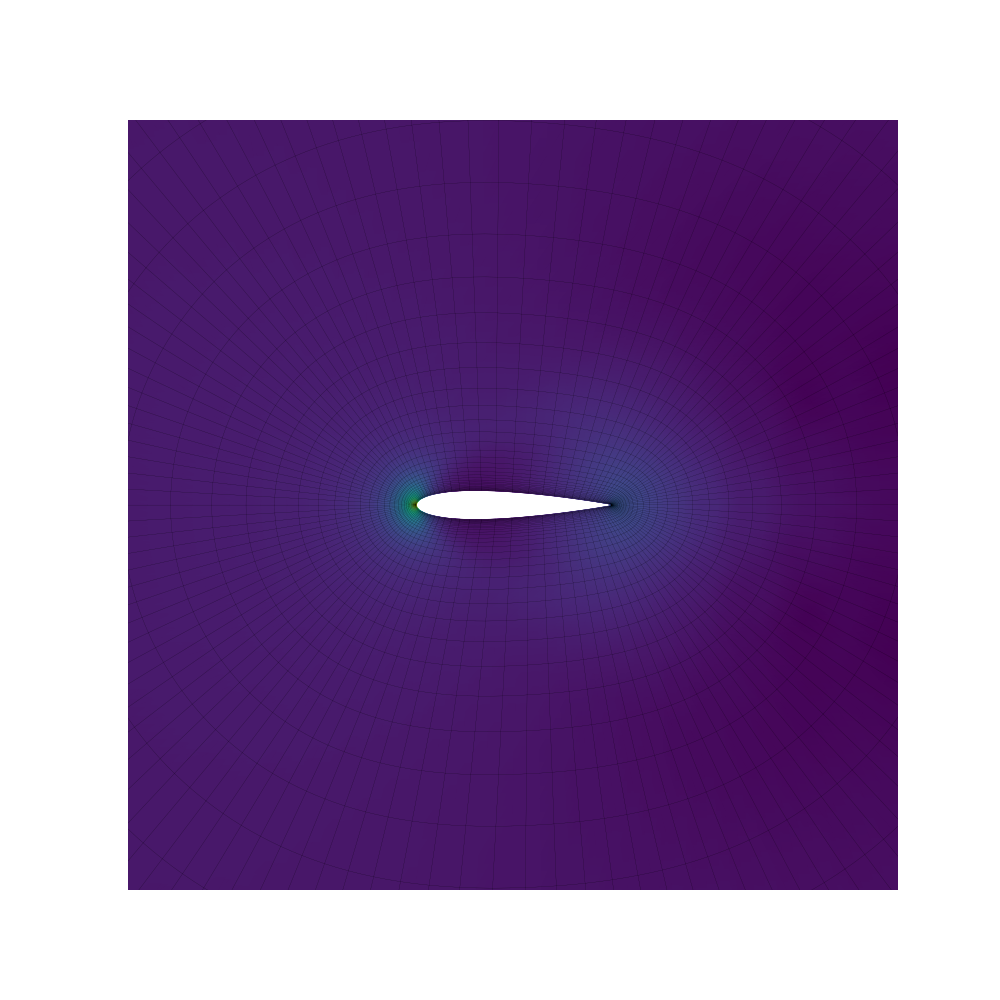
\includegraphics[width=0.4\textwidth]{figs/bfun-p-piola-p004}
    }
    \adjustbox{trim={0.3\width} {0.3\height} {0.3\width} {0.3\height}, clip}{
      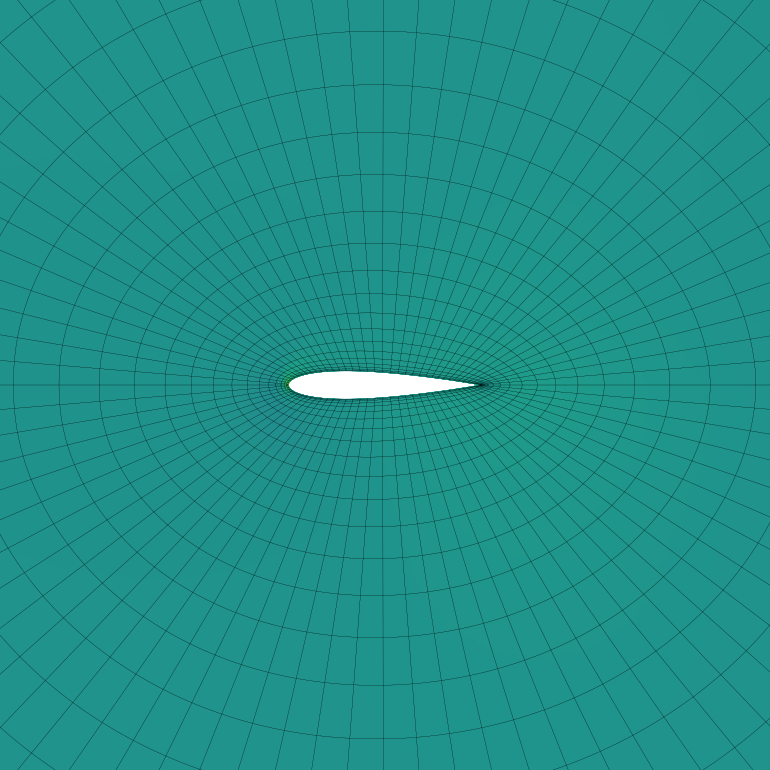
\includegraphics[width=0.4\textwidth]{figs/bfun-p-piola-p005}
    }
    \caption{First six pressure modes (conforming method).}
    \label{fig:modes-press-conf}
  \end{center}
\end{figure}

\begin{figure}
  \begin{center}
    \adjustbox{trim={0.2\width} {0.2\height} {0.2\width} {0.2\height}, clip}{
      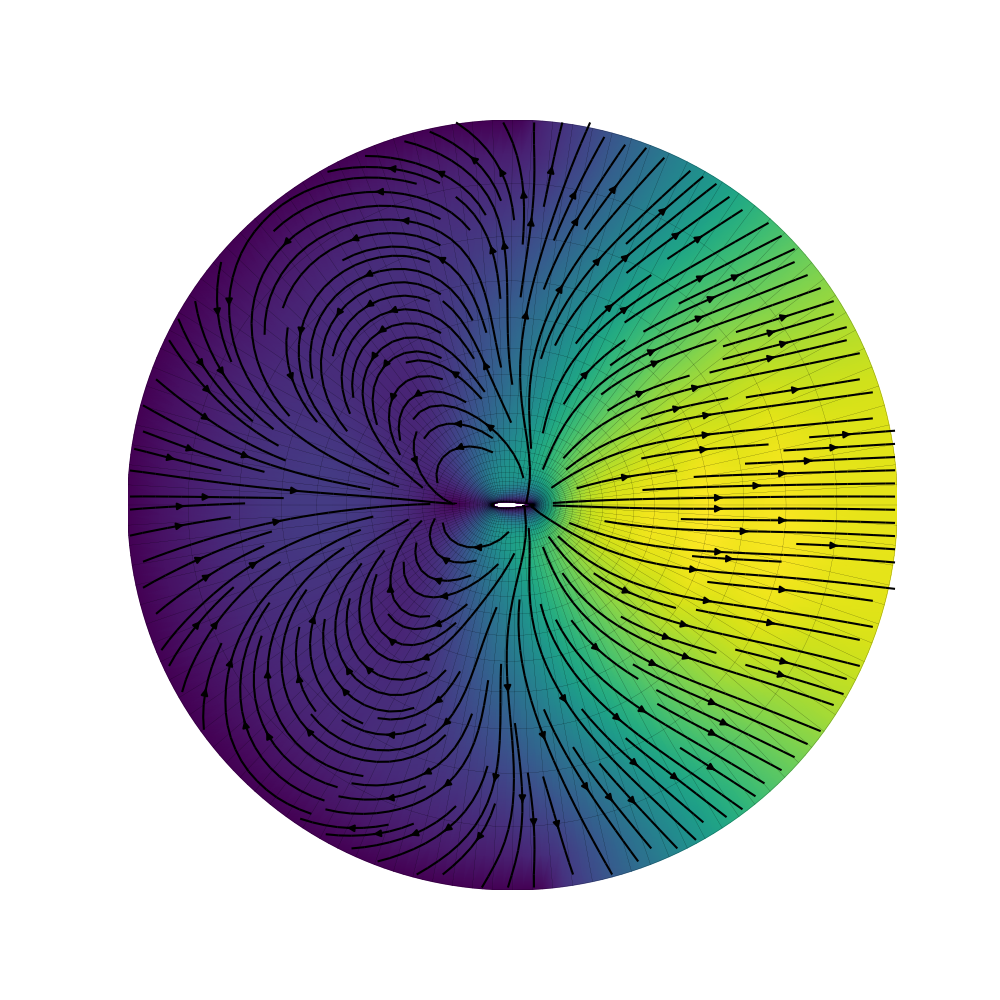
\includegraphics[width=0.4\textwidth]{figs/bfun-s-piola-v000}
    }
    \adjustbox{trim={0.2\width} {0.2\height} {0.2\width} {0.2\height}, clip}{
      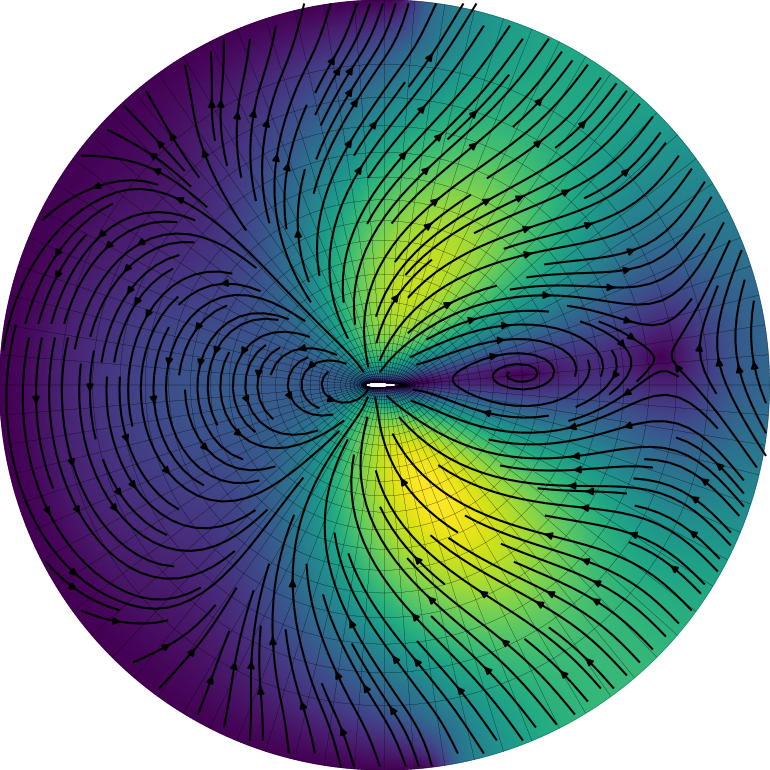
\includegraphics[width=0.4\textwidth]{figs/bfun-s-piola-v001}
    }
    \adjustbox{trim={0.2\width} {0.2\height} {0.2\width} {0.2\height}, clip}{
      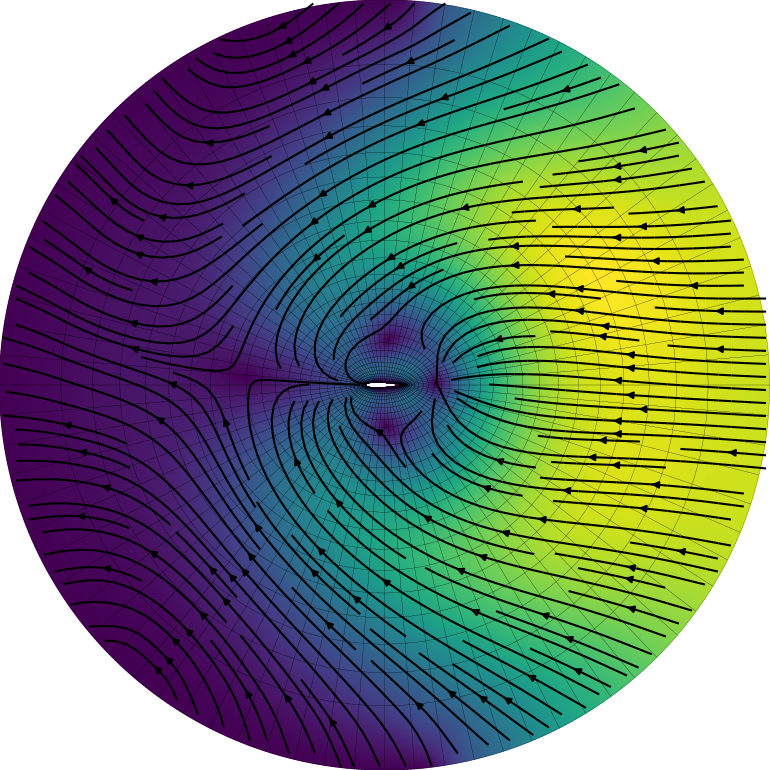
\includegraphics[width=0.4\textwidth]{figs/bfun-s-piola-v002}
    } \\
    \adjustbox{trim={0.2\width} {0.2\height} {0.2\width} {0.2\height}, clip}{
      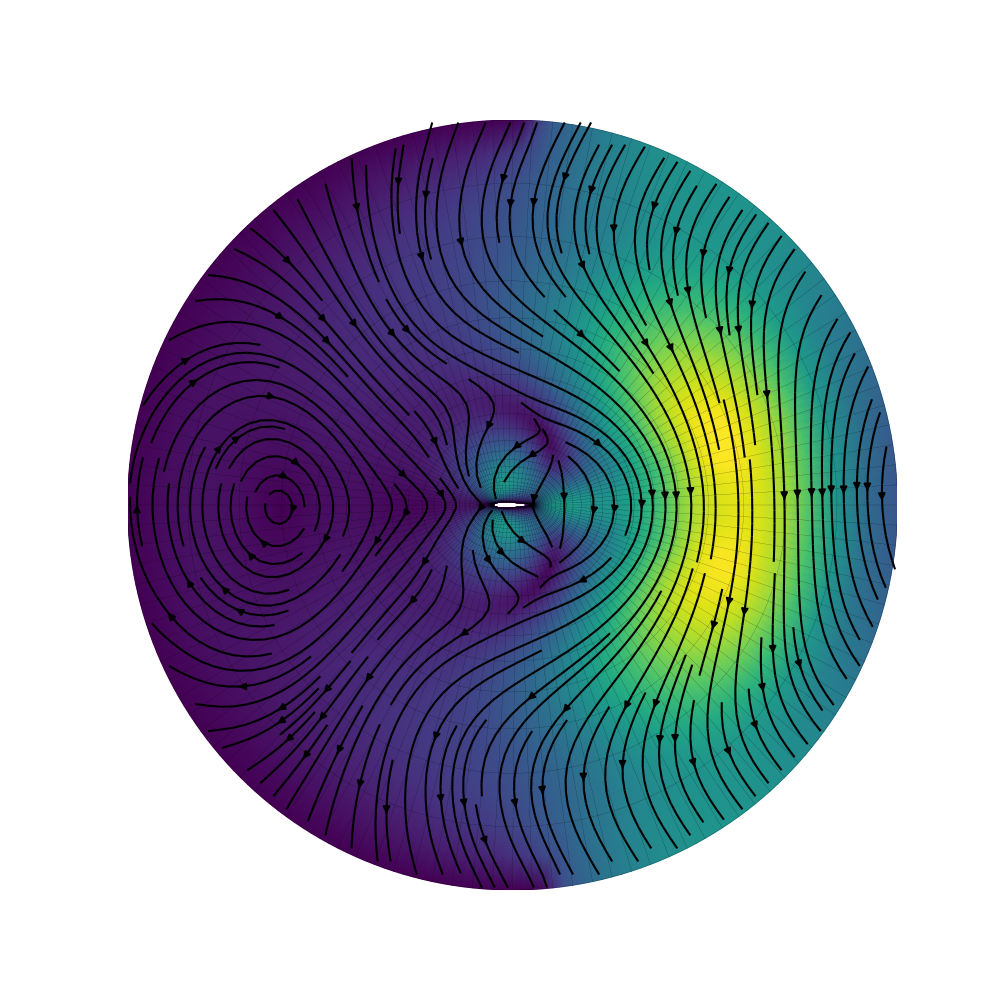
\includegraphics[width=0.4\textwidth]{figs/bfun-s-piola-v003}
    }
    \adjustbox{trim={0.2\width} {0.2\height} {0.2\width} {0.2\height}, clip}{
      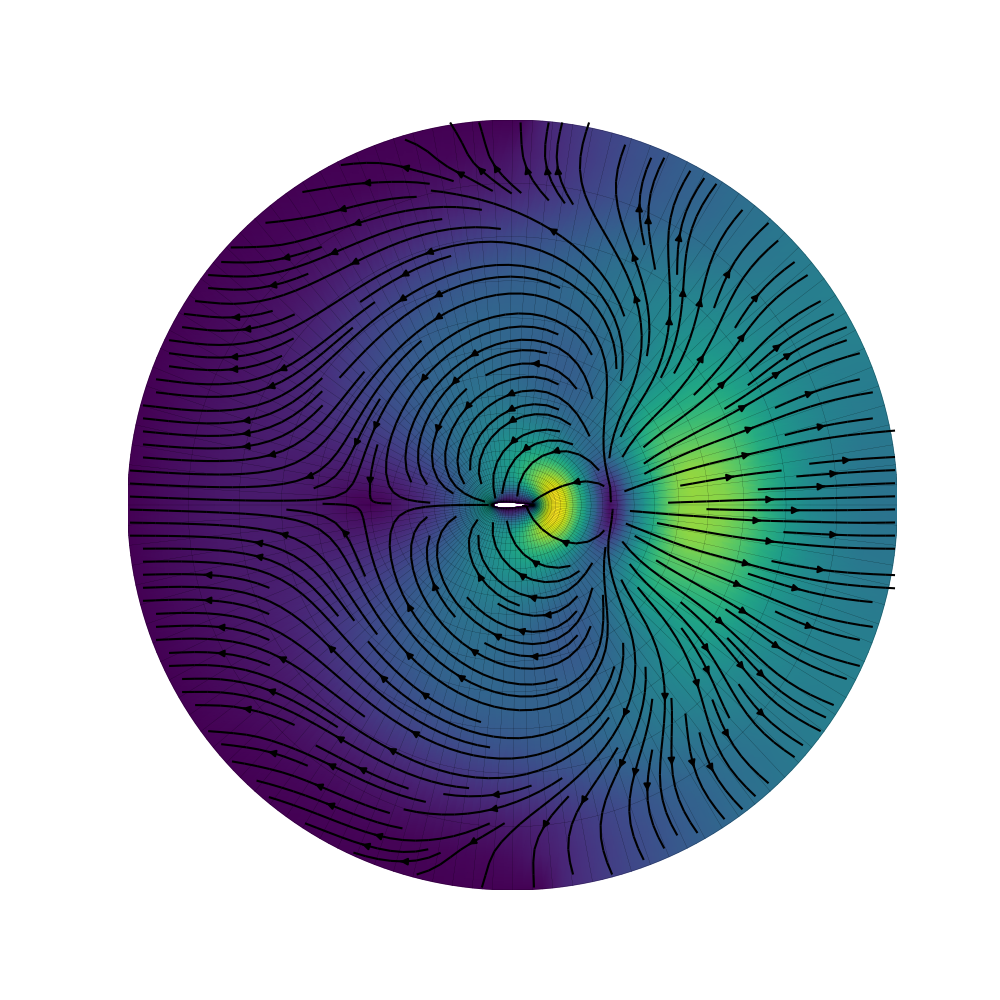
\includegraphics[width=0.4\textwidth]{figs/bfun-s-piola-v004}
    }
    \adjustbox{trim={0.2\width} {0.2\height} {0.2\width} {0.2\height}, clip}{
      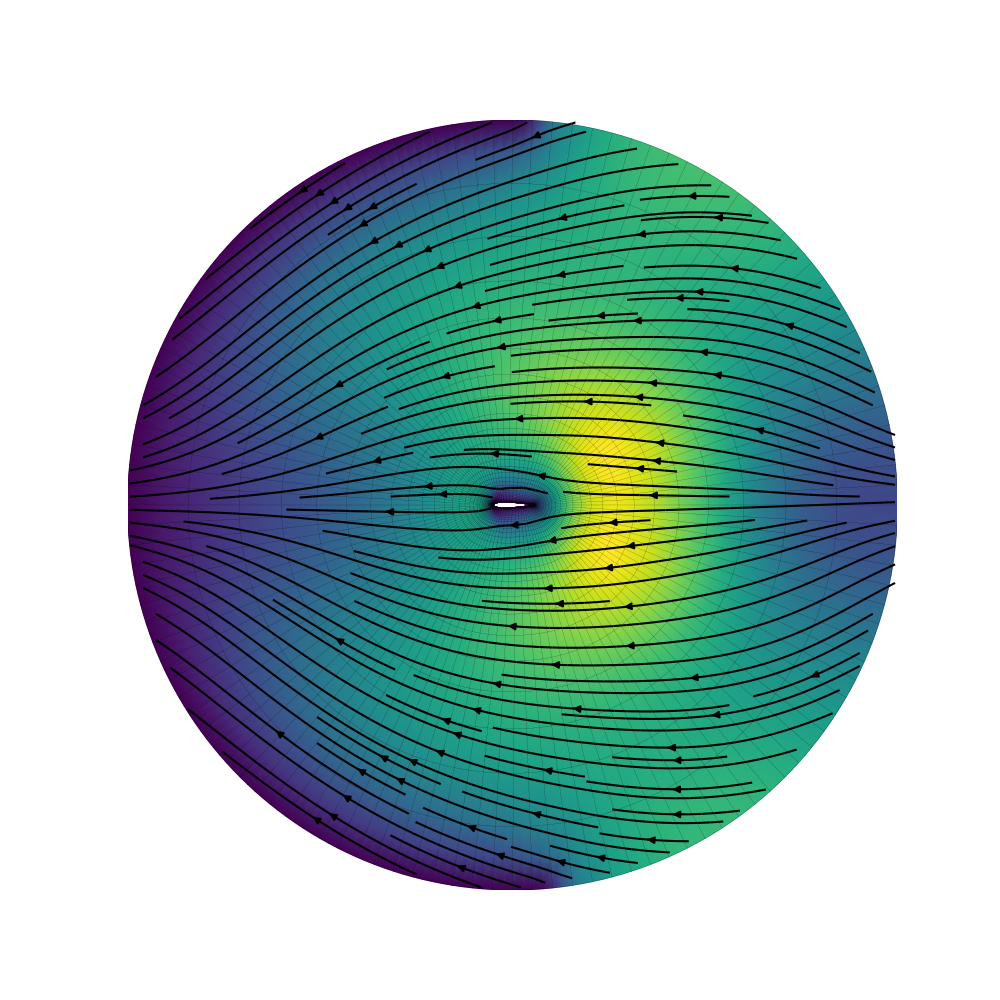
\includegraphics[width=0.4\textwidth]{figs/bfun-s-piola-v005}
    }
    \caption{First six supremizer modes (conforming method).}
    \label{fig:modes-sup-conf}
  \end{center}
\end{figure}

\begin{figure}
  \begin{tikzpicture}
    \begin{axis}[
      xlabel={Angle of attack ($\varphi$, degrees)},
      ylabel={Divergence ($L^2$-norm)},
      ymode=log,
      width=0.9\textwidth,
      height=0.5\textwidth,
      grid=both,
      axis lines=left,
      legend style={
        at={(0.5, -0.2)},
        anchor=north,
        draw=none,
      },
      legend cell align=left,
      legend columns=2,
      ]
      \addplot[blue, thick, mark=*, mark options={solid}]
      table[x index={0}, y index={2}]{data/airfoil-divs-no-piola.csv};
      \addplot[blue, thick, densely dashed, mark=o, mark options={solid}]
      table[x index={0}, y index={1}]{data/airfoil-divs-no-piola.csv};
      \addplot[red, thick, mark=*, mark options={solid}]
      table[x index={0}, y index={2}]{data/airfoil-divs-piola.csv};
      \addplot[red, thick, densely dashed, mark=o, mark options={solid}]
      table[x index={0}, y index={1}]{data/airfoil-divs-piola.csv};
      \legend{
        Regular mean,
        Regular max,
        Conforming mean,
        Conforming max,
      }
    \end{axis}
  \end{tikzpicture}
  \caption{
    Mean and maximal divergences of the ten first basis functions for the
    regular and conforming methods, as measured in $L^2$-norms, for various
    angles of attack.
  }
  \label{fig:divs}
\end{figure}

\subsection{Stability}

To understand the stability properties of the four methods, we computed the LBB
constants $\beta_h$ from \eqref{eqn:lbb}. The results can be seen in
Table~\ref{tbl:lbb}. This clearly demonstrates the ability of the supremizer
enrichment procedure to control the stability of the method. It also highlights
that the conforming method is \emph{generally} somewhat more unstable than the
regular method, but not significantly so.

\begin{table}
  \begin{center}
    \bgroup\def\arraystretch{1.2}
    \begin{tabular}{crrrr}
      & \multicolumn{2}{c}{\bf Regular} & \multicolumn{2}{c}{\bf Conforming} \\
      \hline
      $\sharp$ DoFs ($M$) & \multicolumn{1}{c}{Unstabilized} & \multicolumn{1}{c}{Stabilized} & \multicolumn{1}{c}{Unstabilized} & \multicolumn{1}{c}{Stabilized} \\
      \hline $10$ & $\SI{1.19e-5}{}$ & $\SI{4.07e-1}{}$ & $\SI{4.20e-18}{}$ & $\SI{3.97e-1}{}$ \\
      $20$ & $\SI{9.58e-6}{}$ & $\SI{2.56e-1}{}$ & $\SI{2.80e-19}{}$ & $\SI{2.69e-1}{}$ \\
      $30$ & $\SI{6.44e-7}{}$ & $\SI{3.27e-1}{}$ & $\SI{1.08e-17}{}$ & $\SI{2.86e-1}{}$ \\
      $40$ & $\SI{7.28e-8}{}$ & $\SI{2.81e-1}{}$ & $\SI{2.46e-19}{}$ & $\SI{2.61e-1}{}$ \\
      $50$ & $\SI{1.62e-8}{}$ & $\SI{2.92e-1}{}$ & $\SI{1.42e-18}{}$ & $\SI{2.26e-1}{}$ \\
      \hline
    \end{tabular}
    \egroup
  \end{center}
  \caption{
    LBB constants $\beta_h$, as defined by \eqref{eqn:lbb}, for various basis
    sizes and methods. The reported values are \emph{minima} over a sampling of
    $5 \times 5$ parameter values.
  }
  \label{tbl:lbb}
\end{table}

\subsection{Performance}

Performance metrics are presented in terms of error, speedup and degrees of
freedom.
\begin{itemize}
  \item \emph{Error}, when reported, is always given as
    \emph{mean relative error} between the result of the high-fidelity and the
    reduced basis method. The mean is taken over $25 = 5 \times 5$ uniformly
    spaced points in the parameter space. The error norms used are $H^1$
    seminorm for velocities and $L^2$ norm for pressure. For the regular
    un-stabilized reduced methods, we found that they consistently failed to
    converge, thus the errors reported for those methods are based on fewer
    parameter values (those where convergence could be achieved).
  \item \emph{Expected error} is, given $M$, the smallest $\epsilon$ satisfying
    \eqref{eqn:error}. We used prescribed values of $M=10,20,30,40,50$,
    computing $\epsilon$ as a function of $M$ rather than the other way around.
  \item \emph{Speedup} is the ratio between the mean solution time with the
    high-fidelity model and that of the reduced model. For this metric, all
    relevant matrices and tensors for the high-fidelity modely were
    pre-computed. That is, \emph{no} integration took place within the loop of
    the nonlinear solver. Depending on circumstances, this may be considered
    unusual for high-fidelity solvers, but at any rate can only serve to speed
    them up. In other words, the actual speed gains may realistically be higher
    than reported.
  \item \emph{Degrees of freedom} is the number $M$ of basis functions in a
    \emph{single} reduced space. For the regular method, this implies a total of
    $2M$ degrees of freedom in velocity (although only $M$ of these can be
    expected to have approximative power, the supremizer functions \emph{do}
    contribute to the final solution), and $M$ degrees of freedom in pressure.
    For the conforming method, there are $M$ degrees of freedom in both spaces.
\end{itemize}

Figure~\ref{fig:perf1-unstab} first shows measured error as a function of
expected error, for the stabilized and un-stabilized regular methods. While the
stabilized method can be seen to converge, the velocity solution of the
un-stabilized methods does not, and the pressure solution diverges.

In addition to this, the regular un-stabilized methods has serious convergence
problems, especially for larger $M$, and the conforming un-stabilized methods
essentially never converges for any parameter values. In the following we will
therefore not dwell on the un-stabilized methods.

Figure~\ref{fig:perf1} shows the same results, comparing the regular and the
conforming methods (both stabilized). We see a clear linear relationship between
the expected and mesured errors, as hoped. The conforming method obtains
somewhat better velocity results and comparable pressure results to the regular
method, although the pressure convergence pattern is noticeably more erratic.

The error as a function of degrees of freedom (Figure~\ref{fig:perf2}) tells the
same story.

Figure~\ref{fig:perf3} shows the measured errors as a function of speedup. This
clearly shows the ability of the conforming method to achieve the same results
significantly faster if the block solver algorithm is employed.

\begin{figure}
  \begin{tikzpicture}
    \begin{axis}[
      xlabel={Expected mean relative error},
      ylabel={Mean relative error},
      ymode=log,
      xmode=log,
      width=0.9\textwidth,
      height=0.5\textwidth,
      grid=both,
      axis lines=left,
      legend style={
        at={(0.5, -0.2)},
        anchor=north,
        draw=none,
      },
      legend cell align=left,
      legend columns=2,
      ]
      \addplot[blue, thick, mark=*, mark options={solid}]
      table[x index={1}, y index={4}]{data/airfoil-results-no-piola-sups-no-block.csv};
      \addplot[blue, thick, densely dashed, mark=o, mark options={solid}]
      table[x index={1}, y index={6}]{data/airfoil-results-no-piola-sups-no-block.csv};
      \addplot[magenta, thick, mark=*, mark options={solid}]
      table[x index={1}, y index={4}]{data/airfoil-results-no-piola-no-sups-no-block.csv};
      \addplot[magenta, thick, densely dashed, mark=o, mark options={solid}]
      table[x index={1}, y index={6}]{data/airfoil-results-no-piola-no-sups-no-block.csv};
      \legend{
        Regular stabilized ($v$),
        Regular stabilized ($p$),
        Regular un-stabilized ($v$),
        Regular un-stabilized ($p$),
      }
    \end{axis}
  \end{tikzpicture}
  \caption{
    Measured mean relative error as a function of expected mean relative error,
    for velocity ($H^1$-seminorm) and pressure ($L^2$-norm). The regular
    stabilized and un-stabilized methods are shown. Stabilization is clearly
    necessary to obtain any sort of useful solution.
  }
  \label{fig:perf1-unstab}
\end{figure}

\begin{figure}
  \begin{tikzpicture}
    \begin{axis}[
      xlabel={Expected mean relative error},
      ylabel={Mean relative error},
      ymode=log,
      xmode=log,
      width=0.9\textwidth,
      height=0.5\textwidth,
      grid=both,
      axis lines=left,
      legend style={
        at={(0.5, -0.2)},
        anchor=north,
        draw=none,
      },
      legend cell align=left,
      legend columns=2,
      ]
      \addplot[blue, thick, mark=*, mark options={solid}]
      table[x index={1}, y index={4}]{data/airfoil-results-no-piola-sups-no-block.csv};
      \addplot[blue, thick, densely dashed, mark=o, mark options={solid}]
      table[x index={1}, y index={6}]{data/airfoil-results-no-piola-sups-no-block.csv};
      \addplot[red, thick, mark=*, mark options={solid}]
      table[x index={1}, y index={4}]{data/airfoil-results-piola-sups-no-block.csv};
      \addplot[red, thick, densely dashed, mark=o, mark options={solid}]
      table[x index={1}, y index={6}]{data/airfoil-results-piola-sups-no-block.csv};
      \legend{
        Regular stabilized ($v$),
        Regular stabilized ($p$),
        Conforming stabilized ($v$),
        Conforming stabilized ($p$),
      }
    \end{axis}
  \end{tikzpicture}
  \caption{
    Measured mean relative error as a function of expected mean relative error,
    for velocity ($H^1$-seminorm) and pressure ($L^2$-norm). Both regular and
    conforming are shown. The conforming block solver is indistinguishable from
    the naive conforming solver. Bottom right is better.
  }
  \label{fig:perf1}
\end{figure}

\begin{figure}
  \begin{tikzpicture}
    \begin{axis}[
      xlabel={Degrees of freedom ($M$)},
      ylabel={Mean relative error},
      ymode=log,
      width=0.9\textwidth,
      height=0.5\textwidth,
      grid=both,
      axis lines=left,
      legend style={
        at={(0.5, -0.2)},
        anchor=north,
        draw=none,
      },
      legend cell align=left,
      legend columns=2,
      ]
      \addplot[blue, thick, mark=*, mark options={solid}]
      table[x index={0}, y index={4}]{data/airfoil-results-no-piola-sups-no-block.csv};
      \addplot[blue, thick, densely dashed, mark=o, mark options={solid}]
      table[x index={0}, y index={6}]{data/airfoil-results-no-piola-sups-no-block.csv};
      \addplot[red, thick, mark=*, mark options={solid}]
      table[x index={0}, y index={4}]{data/airfoil-results-piola-sups-no-block.csv};
      \addplot[red, thick, densely dashed, mark=o, mark options={solid}]
      table[x index={0}, y index={6}]{data/airfoil-results-piola-sups-no-block.csv};
      \legend{
        Regular stabilized ($v$),
        Regular stabilized ($p$),
        Conforming stabilized ($v$),
        Conforming stabilized ($p$),
      }
    \end{axis}
  \end{tikzpicture}
  \caption{
    Measured mean relative error as a function of $M$, for velocity
    ($H^1$-seminorm) and pressure ($L^2$-norm). Both regular and conforming are
    shown. The conforming block solver is indistinguishable from the naive
    conforming solver. Bottom left is better.
  }
  \label{fig:perf2}
\end{figure}

\begin{figure}
  \begin{tikzpicture}
    \begin{axis}[
      xlabel={Speedup},
      ylabel={Mean relative error},
      ymode=log,
      xmode=log,
      width=0.9\textwidth,
      height=0.5\textwidth,
      grid=both,
      axis lines=left,
      legend style={
        at={(0.5, -0.2)},
        anchor=north,
        draw=none,
      },
      legend cell align=left,
      legend columns=2,
      ]
      \addplot[blue, thick, mark=*, mark options={solid}]
      table[x index={11}, y index={4}]{data/airfoil-results-no-piola-sups-no-block.csv};
      \addplot[blue, thick, densely dashed, mark=o, mark options={solid}]
      table[x index={11}, y index={6}]{data/airfoil-results-no-piola-sups-no-block.csv};
      \addplot[red, thick, mark=*, mark options={solid}]
      table[x index={11}, y index={4}]{data/airfoil-results-piola-sups-no-block.csv};
      \addplot[red, thick, densely dashed, mark=o, mark options={solid}]
      table[x index={11}, y index={6}]{data/airfoil-results-piola-sups-no-block.csv};
      \addplot[green, thick, mark=*, mark options={solid}]
      table[x index={11}, y index={4}]{data/airfoil-results-piola-sups-block.csv};
      \addplot[green, thick, densely dashed, mark=o, mark options={solid}]
      table[x index={11}, y index={6}]{data/airfoil-results-piola-sups-block.csv};
      \legend{
        Regular stabilized ($v$),
        Regular stabilized ($p$),
        Conforming stabilized naive ($v$),
        Conforming stabilized naive ($p$),
        Conforming stabilized block ($v$),
        Conforming stabilized block ($p$),
      }
    \end{axis}
  \end{tikzpicture}
  \caption{
    Measured mean relative error as a function of speedup, for velocity
    ($H^1$-seminorm) and pressure ($L^2$-norm). Both regular and conforming are
    shown, the latter with two different solvers (the naive solver and the block
    solver). Bottom right is better.
  }
  \label{fig:perf3}
\end{figure}

\section{Conclusions}
\label{sec:conc}

Two methods have been investigated for the parametrized problem of flow around a NACA0015
airfoil with varying angle-of-attack and inflow velocity. One based on a
Taylor-Hood high-fidelity method, and the other based on a divergence-conforming
isogeometric high-fidelity method. The reduced models of both were stabilized
using supremizers \cite{Ballarin2015ssp}.

While the accuracy of the reduced methods were comparable, the
divergence-conforming model was able to achieve a significantly faster online
stage thanks to the block form of its linear systems.

This faster online stage is offset by a more complicated offline stage. In
particular, the affine representations \eqref{eqn:split-1}--\eqref{eqn:split-5}
of the divergence-conforming method required approximately three times as many
terms ($\sim 12n$ versus $\sim 4n$). While the gains in the online stage was not
affected by this, the added complexity in the offline stage should nevertheless
not be taken lightly. It remains to be seen whether automatic ``black box''
methods such as Empirical Interpolation (EIM)
\cite{Barrault2004eim,Grepl2007erb,Maday2007gmi}
\cite[Chapter 10]{Quarteroni2016rbm}
may alleviate this issue.

\bibliography{common/references}
\bibliographystyle{plain}

\end{document}
